% Options for packages loaded elsewhere
\PassOptionsToPackage{unicode}{hyperref}
\PassOptionsToPackage{hyphens}{url}
\PassOptionsToPackage{dvipsnames,svgnames,x11names}{xcolor}
%
\documentclass[
  letterpaper,
  DIV=11,
  numbers=noendperiod]{scrartcl}

\usepackage{amsmath,amssymb}
\usepackage{iftex}
\ifPDFTeX
  \usepackage[T1]{fontenc}
  \usepackage[utf8]{inputenc}
  \usepackage{textcomp} % provide euro and other symbols
\else % if luatex or xetex
  \usepackage{unicode-math}
  \defaultfontfeatures{Scale=MatchLowercase}
  \defaultfontfeatures[\rmfamily]{Ligatures=TeX,Scale=1}
\fi
\usepackage{lmodern}
\ifPDFTeX\else  
    % xetex/luatex font selection
\fi
% Use upquote if available, for straight quotes in verbatim environments
\IfFileExists{upquote.sty}{\usepackage{upquote}}{}
\IfFileExists{microtype.sty}{% use microtype if available
  \usepackage[]{microtype}
  \UseMicrotypeSet[protrusion]{basicmath} % disable protrusion for tt fonts
}{}
\makeatletter
\@ifundefined{KOMAClassName}{% if non-KOMA class
  \IfFileExists{parskip.sty}{%
    \usepackage{parskip}
  }{% else
    \setlength{\parindent}{0pt}
    \setlength{\parskip}{6pt plus 2pt minus 1pt}}
}{% if KOMA class
  \KOMAoptions{parskip=half}}
\makeatother
\usepackage{xcolor}
\setlength{\emergencystretch}{3em} % prevent overfull lines
\setcounter{secnumdepth}{-\maxdimen} % remove section numbering
% Make \paragraph and \subparagraph free-standing
\ifx\paragraph\undefined\else
  \let\oldparagraph\paragraph
  \renewcommand{\paragraph}[1]{\oldparagraph{#1}\mbox{}}
\fi
\ifx\subparagraph\undefined\else
  \let\oldsubparagraph\subparagraph
  \renewcommand{\subparagraph}[1]{\oldsubparagraph{#1}\mbox{}}
\fi

\usepackage{color}
\usepackage{fancyvrb}
\newcommand{\VerbBar}{|}
\newcommand{\VERB}{\Verb[commandchars=\\\{\}]}
\DefineVerbatimEnvironment{Highlighting}{Verbatim}{commandchars=\\\{\}}
% Add ',fontsize=\small' for more characters per line
\usepackage{framed}
\definecolor{shadecolor}{RGB}{241,243,245}
\newenvironment{Shaded}{\begin{snugshade}}{\end{snugshade}}
\newcommand{\AlertTok}[1]{\textcolor[rgb]{0.68,0.00,0.00}{#1}}
\newcommand{\AnnotationTok}[1]{\textcolor[rgb]{0.37,0.37,0.37}{#1}}
\newcommand{\AttributeTok}[1]{\textcolor[rgb]{0.40,0.45,0.13}{#1}}
\newcommand{\BaseNTok}[1]{\textcolor[rgb]{0.68,0.00,0.00}{#1}}
\newcommand{\BuiltInTok}[1]{\textcolor[rgb]{0.00,0.23,0.31}{#1}}
\newcommand{\CharTok}[1]{\textcolor[rgb]{0.13,0.47,0.30}{#1}}
\newcommand{\CommentTok}[1]{\textcolor[rgb]{0.37,0.37,0.37}{#1}}
\newcommand{\CommentVarTok}[1]{\textcolor[rgb]{0.37,0.37,0.37}{\textit{#1}}}
\newcommand{\ConstantTok}[1]{\textcolor[rgb]{0.56,0.35,0.01}{#1}}
\newcommand{\ControlFlowTok}[1]{\textcolor[rgb]{0.00,0.23,0.31}{#1}}
\newcommand{\DataTypeTok}[1]{\textcolor[rgb]{0.68,0.00,0.00}{#1}}
\newcommand{\DecValTok}[1]{\textcolor[rgb]{0.68,0.00,0.00}{#1}}
\newcommand{\DocumentationTok}[1]{\textcolor[rgb]{0.37,0.37,0.37}{\textit{#1}}}
\newcommand{\ErrorTok}[1]{\textcolor[rgb]{0.68,0.00,0.00}{#1}}
\newcommand{\ExtensionTok}[1]{\textcolor[rgb]{0.00,0.23,0.31}{#1}}
\newcommand{\FloatTok}[1]{\textcolor[rgb]{0.68,0.00,0.00}{#1}}
\newcommand{\FunctionTok}[1]{\textcolor[rgb]{0.28,0.35,0.67}{#1}}
\newcommand{\ImportTok}[1]{\textcolor[rgb]{0.00,0.46,0.62}{#1}}
\newcommand{\InformationTok}[1]{\textcolor[rgb]{0.37,0.37,0.37}{#1}}
\newcommand{\KeywordTok}[1]{\textcolor[rgb]{0.00,0.23,0.31}{#1}}
\newcommand{\NormalTok}[1]{\textcolor[rgb]{0.00,0.23,0.31}{#1}}
\newcommand{\OperatorTok}[1]{\textcolor[rgb]{0.37,0.37,0.37}{#1}}
\newcommand{\OtherTok}[1]{\textcolor[rgb]{0.00,0.23,0.31}{#1}}
\newcommand{\PreprocessorTok}[1]{\textcolor[rgb]{0.68,0.00,0.00}{#1}}
\newcommand{\RegionMarkerTok}[1]{\textcolor[rgb]{0.00,0.23,0.31}{#1}}
\newcommand{\SpecialCharTok}[1]{\textcolor[rgb]{0.37,0.37,0.37}{#1}}
\newcommand{\SpecialStringTok}[1]{\textcolor[rgb]{0.13,0.47,0.30}{#1}}
\newcommand{\StringTok}[1]{\textcolor[rgb]{0.13,0.47,0.30}{#1}}
\newcommand{\VariableTok}[1]{\textcolor[rgb]{0.07,0.07,0.07}{#1}}
\newcommand{\VerbatimStringTok}[1]{\textcolor[rgb]{0.13,0.47,0.30}{#1}}
\newcommand{\WarningTok}[1]{\textcolor[rgb]{0.37,0.37,0.37}{\textit{#1}}}

\providecommand{\tightlist}{%
  \setlength{\itemsep}{0pt}\setlength{\parskip}{0pt}}\usepackage{longtable,booktabs,array}
\usepackage{calc} % for calculating minipage widths
% Correct order of tables after \paragraph or \subparagraph
\usepackage{etoolbox}
\makeatletter
\patchcmd\longtable{\par}{\if@noskipsec\mbox{}\fi\par}{}{}
\makeatother
% Allow footnotes in longtable head/foot
\IfFileExists{footnotehyper.sty}{\usepackage{footnotehyper}}{\usepackage{footnote}}
\makesavenoteenv{longtable}
\usepackage{graphicx}
\makeatletter
\def\maxwidth{\ifdim\Gin@nat@width>\linewidth\linewidth\else\Gin@nat@width\fi}
\def\maxheight{\ifdim\Gin@nat@height>\textheight\textheight\else\Gin@nat@height\fi}
\makeatother
% Scale images if necessary, so that they will not overflow the page
% margins by default, and it is still possible to overwrite the defaults
% using explicit options in \includegraphics[width, height, ...]{}
\setkeys{Gin}{width=\maxwidth,height=\maxheight,keepaspectratio}
% Set default figure placement to htbp
\makeatletter
\def\fps@figure{htbp}
\makeatother

<script src="Part1_Lecture1_Ex_files/libs/htmlwidgets-1.6.4/htmlwidgets.js"></script>
<script src="Part1_Lecture1_Ex_files/libs/plotly-binding-4.10.4/plotly.js"></script>
<script src="Part1_Lecture1_Ex_files/libs/setprototypeof-0.1/setprototypeof.js"></script>
<script src="Part1_Lecture1_Ex_files/libs/typedarray-0.1/typedarray.min.js"></script>
<script src="Part1_Lecture1_Ex_files/libs/jquery-3.5.1/jquery.min.js"></script>
<link href="Part1_Lecture1_Ex_files/libs/crosstalk-1.2.1/css/crosstalk.min.css" rel="stylesheet" />
<script src="Part1_Lecture1_Ex_files/libs/crosstalk-1.2.1/js/crosstalk.min.js"></script>
<link href="Part1_Lecture1_Ex_files/libs/plotly-htmlwidgets-css-2.11.1/plotly-htmlwidgets.css" rel="stylesheet" />
<script src="Part1_Lecture1_Ex_files/libs/plotly-main-2.11.1/plotly-latest.min.js"></script>
\KOMAoption{captions}{tableheading}
\makeatletter
\makeatother
\makeatletter
\makeatother
\makeatletter
\@ifpackageloaded{caption}{}{\usepackage{caption}}
\AtBeginDocument{%
\ifdefined\contentsname
  \renewcommand*\contentsname{Table of contents}
\else
  \newcommand\contentsname{Table of contents}
\fi
\ifdefined\listfigurename
  \renewcommand*\listfigurename{List of Figures}
\else
  \newcommand\listfigurename{List of Figures}
\fi
\ifdefined\listtablename
  \renewcommand*\listtablename{List of Tables}
\else
  \newcommand\listtablename{List of Tables}
\fi
\ifdefined\figurename
  \renewcommand*\figurename{Figure}
\else
  \newcommand\figurename{Figure}
\fi
\ifdefined\tablename
  \renewcommand*\tablename{Table}
\else
  \newcommand\tablename{Table}
\fi
}
\@ifpackageloaded{float}{}{\usepackage{float}}
\floatstyle{ruled}
\@ifundefined{c@chapter}{\newfloat{codelisting}{h}{lop}}{\newfloat{codelisting}{h}{lop}[chapter]}
\floatname{codelisting}{Listing}
\newcommand*\listoflistings{\listof{codelisting}{List of Listings}}
\makeatother
\makeatletter
\@ifpackageloaded{caption}{}{\usepackage{caption}}
\@ifpackageloaded{subcaption}{}{\usepackage{subcaption}}
\makeatother
\makeatletter
\@ifpackageloaded{tcolorbox}{}{\usepackage[skins,breakable]{tcolorbox}}
\makeatother
\makeatletter
\@ifundefined{shadecolor}{\definecolor{shadecolor}{rgb}{.97, .97, .97}}
\makeatother
\makeatletter
\makeatother
\makeatletter
\makeatother
\ifLuaTeX
  \usepackage{selnolig}  % disable illegal ligatures
\fi
\IfFileExists{bookmark.sty}{\usepackage{bookmark}}{\usepackage{hyperref}}
\IfFileExists{xurl.sty}{\usepackage{xurl}}{} % add URL line breaks if available
\urlstyle{same} % disable monospaced font for URLs
\hypersetup{
  pdftitle={R for Data Analytics Part 1, Lecture 1},
  pdfauthor={Michèle Fille},
  colorlinks=true,
  linkcolor={blue},
  filecolor={Maroon},
  citecolor={Blue},
  urlcolor={Blue},
  pdfcreator={LaTeX via pandoc}}

\title{R for Data Analytics Part 1, Lecture 1}
\author{Michèle Fille}
\date{}

\begin{document}
\maketitle
\ifdefined\Shaded\renewenvironment{Shaded}{\begin{tcolorbox}[frame hidden, enhanced, borderline west={3pt}{0pt}{shadecolor}, interior hidden, breakable, boxrule=0pt, sharp corners]}{\end{tcolorbox}}\fi

\renewcommand*\contentsname{Table of contents}
{
\hypersetup{linkcolor=}
\setcounter{tocdepth}{4}
\tableofcontents
}
\hypertarget{lecture-1---basics-and-plotting}{%
\section{Lecture 1 - Basics and
Plotting}\label{lecture-1---basics-and-plotting}}

\hypertarget{a-quick-tour-of-r-and-rstudio}{%
\subsection{1.1 A Quick Tour of R and
RStudio}\label{a-quick-tour-of-r-and-rstudio}}

\hypertarget{exercise-1.1.-the-basics}{%
\subsubsection{Exercise 1.1. The
Basics}\label{exercise-1.1.-the-basics}}

\hypertarget{exercise-1.1-task-1-magic-with-numbers}{%
\paragraph{Exercise 1.1 -- Task 1: Magic with
numbers}\label{exercise-1.1-task-1-magic-with-numbers}}

Execute in the Console window the following mathematical operations. If
you execute everything correctly, you should end up with the same number
that you started with!

\begin{enumerate}
\def\labelenumi{\arabic{enumi}.}
\item
  Choose any number and add 2 to it.
\item
  Multiply the result by 3.
\item
  Subtract 6 from the answer.
\item
  Divide what you get by 3.
\end{enumerate}

\begin{Shaded}
\begin{Highlighting}[]
\NormalTok{step1 }\OtherTok{\textless{}{-}} \DecValTok{7} \SpecialCharTok{+} \DecValTok{2}      \CommentTok{\# = 9}
\NormalTok{step2 }\OtherTok{\textless{}{-}}\NormalTok{ step1 }\SpecialCharTok{*} \DecValTok{3}  \CommentTok{\# = 27}
\NormalTok{step3 }\OtherTok{\textless{}{-}}\NormalTok{ step2 }\SpecialCharTok{{-}} \DecValTok{6}  \CommentTok{\# = 21}
\NormalTok{step4 }\OtherTok{\textless{}{-}}\NormalTok{ step3 }\SpecialCharTok{/} \DecValTok{3}  \CommentTok{\# = 7}
\NormalTok{step4}
\end{Highlighting}
\end{Shaded}

\begin{verbatim}
[1] 7
\end{verbatim}

\begin{Shaded}
\begin{Highlighting}[]
\CommentTok{\#or}
\NormalTok{(((}\DecValTok{7}\SpecialCharTok{+}\DecValTok{2}\NormalTok{)}\SpecialCharTok{*}\DecValTok{3}\NormalTok{)}\SpecialCharTok{{-}}\DecValTok{6}\NormalTok{)}\SpecialCharTok{/}\DecValTok{3}
\end{Highlighting}
\end{Shaded}

\begin{verbatim}
[1] 7
\end{verbatim}

\hypertarget{exercise-1.1-task-2-create-an-r-skript}{%
\paragraph{Exercise 1.1 -- Task 2: Create an
R-skript}\label{exercise-1.1-task-2-create-an-r-skript}}

\begin{itemize}
\item
  Create a new \textbf{folder} „Lecture\_1`` on your computer.
\item
  Create a new \textbf{R-project} in that folder.
\item
  Create as new \textbf{R-skript} in that project.
\item
  Recreate the \textbf{display} on the right (see:
  Figure~\ref{fig-desired-output} and for solution
  Figure~\ref{fig-mpg-geom-point}.
\end{itemize}

\begin{figure}

{\centering \includegraphics{Materials L1/Exercise 1.1 – Task 2 Create an R-skript.PNG}

}

\caption{\label{fig-desired-output}Desired Output}

\end{figure}

Note:

\begin{itemize}
\item
  Don`t forget to install the ggplot2 package before loading it.
\item
  The operator \textless- assigns the plot output to a variable
  (mpg\_plot).
\item
  The data set mpg is automatically loaded together with ggplot2. Use
  ?mpg to see what it is about.
\end{itemize}

Note:

\begin{itemize}
\tightlist
\item
  To execute a command in the Source pane, press Strg+Enter (Windows) or
  command+Enter (Mac).
\end{itemize}

Remark:

\begin{itemize}
\tightlist
\item
  It is helpful to make a new R Project in a new folder for each major
  project you start in on.
\end{itemize}

\begin{Shaded}
\begin{Highlighting}[]
\CommentTok{\# install.packages("ggplot2") \# already installed}
\FunctionTok{library}\NormalTok{(ggplot2)}
\NormalTok{mpg\_plot }\OtherTok{\textless{}{-}} \FunctionTok{ggplot}\NormalTok{(mpg, }\FunctionTok{aes}\NormalTok{(}\AttributeTok{x =}\NormalTok{ displ, }\AttributeTok{y =}\NormalTok{ hwy)) }\SpecialCharTok{+} \FunctionTok{geom\_point}\NormalTok{(}\FunctionTok{aes}\NormalTok{(}\AttributeTok{colour =}\NormalTok{ class))}

\NormalTok{mpg\_plot}
\end{Highlighting}
\end{Shaded}

\begin{figure}[H]

{\centering 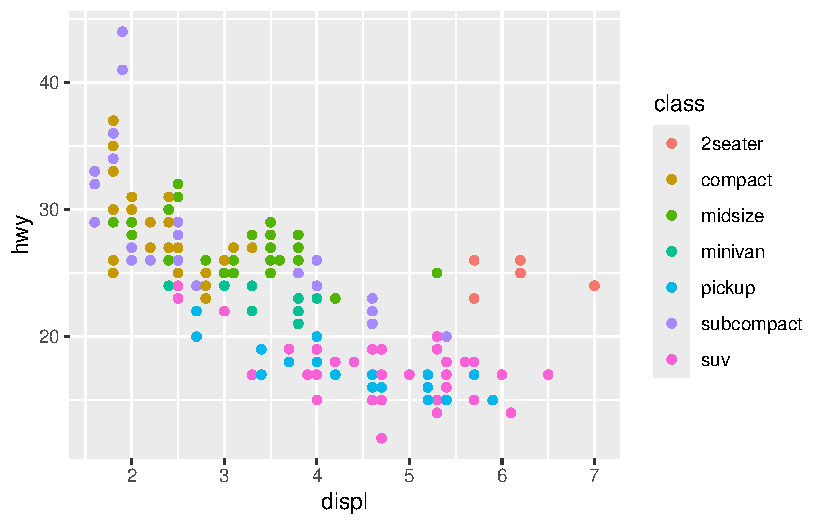
\includegraphics{Part1_Lecture1_Ex_files/figure-pdf/fig-mpg-geom-point-1.pdf}

}

\caption{\label{fig-mpg-geom-point}Scatterplot of Fuel economy data from
1999 to 2008 for 38 popular models of cars}

\end{figure}

\hypertarget{exercise-1.1-task-3-load-a-csv-file-with-base-r}{%
\paragraph{Exercise 1.1 -- Task 3: Load a csv file with base
R}\label{exercise-1.1-task-3-load-a-csv-file-with-base-r}}

\begin{enumerate}
\def\labelenumi{\arabic{enumi}.}
\item
  Install and load the libraries readr and data.table.
\item
  Download the dataset \textbf{female\_names.csv} from Moodle.
\item
  Load the data set into R using \emph{read\_csv()} from base R.
  \textbf{Store it in a variable fnames}. To do that, use \textbf{the
  assignment operator \textless-} : \emph{fnames \textless-
  read.csv(``female\_names.csv'')}
\item
  To get a first impression of the data set, type \textbf{View(fnames)}.
  Alternatively, you can click on the variable name in the Environments
  pane.
\item
  Now load it again,
\end{enumerate}

\begin{itemize}
\item
  using \emph{read.csv()} from package readr, and store it in the
  variable fnames1.
\item
  using \emph{fread()}, from from package data.table, and store it in
  the variable fnames2.
\end{itemize}

Do you experience a difference in performance?

\begin{Shaded}
\begin{Highlighting}[]
\CommentTok{\#install.packages("readr") \# already installed}
\CommentTok{\#install.packages("data.table") \# already installed}
\FunctionTok{library}\NormalTok{(readr)}
\FunctionTok{library}\NormalTok{(data.table)}

\NormalTok{fnames }\OtherTok{\textless{}{-}} \FunctionTok{read\_csv}\NormalTok{(}\StringTok{"\textasciitilde{}/Michele\_FHNW/Semester\_8/Time Series Analysis with R/R\_Files/Summary/Materials L1/female\_names.csv"}\NormalTok{)}
\end{Highlighting}
\end{Shaded}

\begin{verbatim}
Error: '~/Michele_FHNW/Semester_8/Time Series Analysis with R/R_Files/Summary/Materials L1/female_names.csv' does not exist.
\end{verbatim}

\begin{Shaded}
\begin{Highlighting}[]
\FunctionTok{View}\NormalTok{(fnames)}
\end{Highlighting}
\end{Shaded}

\begin{verbatim}
Error in eval(expr, envir, enclos): Objekt 'fnames' nicht gefunden
\end{verbatim}

\begin{Shaded}
\begin{Highlighting}[]
\NormalTok{fnames1 }\OtherTok{\textless{}{-}} \FunctionTok{read.csv}\NormalTok{(}\StringTok{"\textasciitilde{}/Michele\_FHNW/Semester\_8/Time Series Analysis with R/R\_Files/Summary/Materials L1/female\_names.csv"}\NormalTok{)}
\end{Highlighting}
\end{Shaded}

\begin{verbatim}
Warning in file(file, "rt"): kann Datei
'C:/Users/miche/Documents/Michele_FHNW/Semester_8/Time Series Analysis with
R/R_Files/Summary/Materials L1/female_names.csv' nicht öffnen: No such file or
directory
\end{verbatim}

\begin{verbatim}
Error in file(file, "rt"): kann Verbindung nicht öffnen
\end{verbatim}

\begin{Shaded}
\begin{Highlighting}[]
\NormalTok{fnames2 }\OtherTok{\textless{}{-}} \FunctionTok{fread}\NormalTok{(}\StringTok{"\textasciitilde{}/Michele\_FHNW/Semester\_8/Time Series Analysis with R/R\_Files/Summary/Materials L1/female\_names.csv"}\NormalTok{)}
\end{Highlighting}
\end{Shaded}

\begin{verbatim}
Warning in (if (.Platform$OS.type == "unix") system else shell)(paste0("(", :
'(~/Michele_FHNW/Semester_8/Time Series Analysis with
R/R_Files/Summary/Materials L1/female_names.csv) >
C:\Users\miche\AppData\Local\Temp\Rtmpic8ZJN\file34ac55f340e' Ausführung mit
Fehlerkode 1 fehlgeschlagen
\end{verbatim}

\begin{verbatim}
Warning: File 'C:\Users\miche\AppData\Local\Temp\Rtmpic8ZJN\file34ac55f340e'
has size 0. Returning a NULL data.table.
\end{verbatim}

\hypertarget{exercise-1.1-task-4-work-with-data-types}{%
\paragraph{Exercise 1.1 -- Task 4: Work with Data
Types}\label{exercise-1.1-task-4-work-with-data-types}}

What is the data type of each of the following objects. If you don't
know, check the type using \emph{typeof()}.

\begin{itemize}
\item
  1
\item
  5L
\item
  sqrt(-1 +0i)
\item
  ``25''
\end{itemize}

\begin{Shaded}
\begin{Highlighting}[]
\FunctionTok{typeof}\NormalTok{(}\DecValTok{1}\NormalTok{)  }\CommentTok{\# double}
\end{Highlighting}
\end{Shaded}

\begin{verbatim}
[1] "double"
\end{verbatim}

\begin{Shaded}
\begin{Highlighting}[]
\FunctionTok{typeof}\NormalTok{(5L) }\CommentTok{\# integer}
\end{Highlighting}
\end{Shaded}

\begin{verbatim}
[1] "integer"
\end{verbatim}

\begin{Shaded}
\begin{Highlighting}[]
\FunctionTok{typeof}\NormalTok{(}\FunctionTok{sqrt}\NormalTok{(}\SpecialCharTok{{-}}\DecValTok{1}\SpecialCharTok{+}\NormalTok{0i)) }\CommentTok{\#complex}
\end{Highlighting}
\end{Shaded}

\begin{verbatim}
[1] "complex"
\end{verbatim}

\begin{Shaded}
\begin{Highlighting}[]
\FunctionTok{typeof}\NormalTok{(}\StringTok{"25"}\NormalTok{) }\CommentTok{\# character}
\end{Highlighting}
\end{Shaded}

\begin{verbatim}
[1] "character"
\end{verbatim}

Which of these coercions work? What do they produce?

\begin{itemize}
\item
  as.numeric(FALSE)
\item
  as.logical(``Hello!'')
\item
  as.integer(4.4)
\item
  as.character(TRUE)
\item
  as.numeric(``scooby snacks'')
\end{itemize}

\begin{Shaded}
\begin{Highlighting}[]
\FunctionTok{as.numeric}\NormalTok{(}\ConstantTok{FALSE}\NormalTok{) }\CommentTok{\# 0}
\end{Highlighting}
\end{Shaded}

\begin{verbatim}
[1] 0
\end{verbatim}

\begin{Shaded}
\begin{Highlighting}[]
\FunctionTok{as.logical}\NormalTok{(}\StringTok{"Hello!"}\NormalTok{) }\CommentTok{\# NA}
\end{Highlighting}
\end{Shaded}

\begin{verbatim}
[1] NA
\end{verbatim}

\begin{Shaded}
\begin{Highlighting}[]
\FunctionTok{as.integer}\NormalTok{(}\FloatTok{4.4}\NormalTok{) }\CommentTok{\# 4}
\end{Highlighting}
\end{Shaded}

\begin{verbatim}
[1] 4
\end{verbatim}

\begin{Shaded}
\begin{Highlighting}[]
\FunctionTok{as.character}\NormalTok{(}\ConstantTok{TRUE}\NormalTok{) }\CommentTok{\# "TRUE"}
\end{Highlighting}
\end{Shaded}

\begin{verbatim}
[1] "TRUE"
\end{verbatim}

\begin{Shaded}
\begin{Highlighting}[]
\FunctionTok{as.numeric}\NormalTok{(}\StringTok{"scooby snacks"}\NormalTok{) }\CommentTok{\# NA}
\end{Highlighting}
\end{Shaded}

\begin{verbatim}
Warning: NAs durch Umwandlung erzeugt
\end{verbatim}

\begin{verbatim}
[1] NA
\end{verbatim}

What is the output of each of these lines of code? Why?

\begin{itemize}
\item
  sqrt(-1)
\item
  ``1'' + ``5''
\item
  1 + 7
\item
  TRUE + FALSE
\end{itemize}

\begin{Shaded}
\begin{Highlighting}[]
\FunctionTok{sqrt}\NormalTok{(}\SpecialCharTok{{-}}\DecValTok{1}\NormalTok{) }\CommentTok{\# NaN (Not a Number {-}\textgreater{} is a complex number, to make it clear sqrt({-}1+0i))}
\end{Highlighting}
\end{Shaded}

\begin{verbatim}
Warning in sqrt(-1): NaNs wurden erzeugt
\end{verbatim}

\begin{verbatim}
[1] NaN
\end{verbatim}

\begin{Shaded}
\begin{Highlighting}[]
\StringTok{"1"} \SpecialCharTok{+} \StringTok{"5"} \CommentTok{\# Error: strings cannot be conncatenated with +}
\end{Highlighting}
\end{Shaded}

\begin{verbatim}
Error in "1" + "5": nicht-numerisches Argument für binären Operator
\end{verbatim}

\begin{Shaded}
\begin{Highlighting}[]
\DecValTok{1} \SpecialCharTok{+} \DecValTok{7} \CommentTok{\# 8}
\end{Highlighting}
\end{Shaded}

\begin{verbatim}
[1] 8
\end{verbatim}

\begin{Shaded}
\begin{Highlighting}[]
\ConstantTok{TRUE} \SpecialCharTok{+} \ConstantTok{FALSE} \CommentTok{\# 1, cz logic can be coerced (gezwungen) to numeric}
\end{Highlighting}
\end{Shaded}

\begin{verbatim}
[1] 1
\end{verbatim}

\hypertarget{exercise-1.1-task-5-work-with-data-structures}{%
\paragraph{Exercise 1.1 -- Task 5: Work with Data
Structures}\label{exercise-1.1-task-5-work-with-data-structures}}

Create a vector of integers of length 20 and store it in the variable v.

\begin{Shaded}
\begin{Highlighting}[]
\NormalTok{v }\OtherTok{\textless{}{-}} \DecValTok{1}\SpecialCharTok{:}\DecValTok{20}
\NormalTok{v}
\end{Highlighting}
\end{Shaded}

\begin{verbatim}
 [1]  1  2  3  4  5  6  7  8  9 10 11 12 13 14 15 16 17 18 19 20
\end{verbatim}

Use your vector v to create a matrix of integers with dimensions 4x5 and
store it in the variable m.

\begin{Shaded}
\begin{Highlighting}[]
\NormalTok{m }\OtherTok{\textless{}{-}} \FunctionTok{matrix}\NormalTok{(v,}\AttributeTok{nrow =} \DecValTok{4}\NormalTok{)}
\NormalTok{m}
\end{Highlighting}
\end{Shaded}

\begin{verbatim}
     [,1] [,2] [,3] [,4] [,5]
[1,]    1    5    9   13   17
[2,]    2    6   10   14   18
[3,]    3    7   11   15   19
[4,]    4    8   12   16   20
\end{verbatim}

Coerce your matrix m into a data frame and store the result in the
variable df.

\begin{Shaded}
\begin{Highlighting}[]
\NormalTok{df }\OtherTok{\textless{}{-}} \FunctionTok{as.data.frame}\NormalTok{(m)}
\NormalTok{df}
\end{Highlighting}
\end{Shaded}

\begin{verbatim}
  V1 V2 V3 V4 V5
1  1  5  9 13 17
2  2  6 10 14 18
3  3  7 11 15 19
4  4  8 12 16 20
\end{verbatim}

Create a list called my\_list with the following 4 elements:

\begin{itemize}
\item
  ``I love summer''
\item
  TRUE
\item
  ``fun temperatures''
\item
  c(24,25,26)
\end{itemize}

\begin{Shaded}
\begin{Highlighting}[]
\NormalTok{my\_list }\OtherTok{\textless{}{-}} \FunctionTok{list}\NormalTok{(}\StringTok{"I love summer"}\NormalTok{, }\ConstantTok{TRUE}\NormalTok{, }\StringTok{"fun temperatures"}\NormalTok{, }\FunctionTok{c}\NormalTok{(}\DecValTok{24}\NormalTok{,}\DecValTok{25}\NormalTok{,}\DecValTok{26}\NormalTok{))}
\NormalTok{my\_list}
\end{Highlighting}
\end{Shaded}

\begin{verbatim}
[[1]]
[1] "I love summer"

[[2]]
[1] TRUE

[[3]]
[1] "fun temperatures"

[[4]]
[1] 24 25 26
\end{verbatim}

Create a data frame with the following columns (vectors) and save it in
the variable my\_df:

\begin{itemize}
\item
  Your name and the name of your 2 best friends.
\item
  Your age and your 2 best friends' ages.
\item
  Whether you and each of your 2 friends own a car or not (as Boolean
  values).
\end{itemize}

\begin{Shaded}
\begin{Highlighting}[]
\NormalTok{names }\OtherTok{\textless{}{-}} \FunctionTok{c}\NormalTok{(}\StringTok{"Michele"}\NormalTok{, }\StringTok{"Pelin"}\NormalTok{, }\StringTok{"Selina"}\NormalTok{)}
\NormalTok{ages }\OtherTok{\textless{}{-}} \FunctionTok{c}\NormalTok{(}\DecValTok{28}\NormalTok{,}\DecValTok{29}\NormalTok{,}\DecValTok{28}\NormalTok{)}
\NormalTok{cars }\OtherTok{\textless{}{-}} \FunctionTok{c}\NormalTok{(}\ConstantTok{TRUE}\NormalTok{, }\ConstantTok{TRUE}\NormalTok{, }\ConstantTok{TRUE}\NormalTok{)}

\NormalTok{my\_df }\OtherTok{\textless{}{-}} \FunctionTok{data.frame}\NormalTok{(names, ages, cars)}
\NormalTok{my\_df}
\end{Highlighting}
\end{Shaded}

\begin{verbatim}
    names ages cars
1 Michele   28 TRUE
2   Pelin   29 TRUE
3  Selina   28 TRUE
\end{verbatim}

\begin{Shaded}
\begin{Highlighting}[]
\CommentTok{\# or}

\NormalTok{my\_df1 }\OtherTok{\textless{}{-}} \FunctionTok{data.frame}\NormalTok{(}\AttributeTok{names =} \FunctionTok{c}\NormalTok{(}\StringTok{"Michele"}\NormalTok{, }\StringTok{"Noe"}\NormalTok{, }\StringTok{"Pariya"}\NormalTok{),}
                    \AttributeTok{ages =} \FunctionTok{c}\NormalTok{(}\DecValTok{28}\NormalTok{, }\DecValTok{22}\NormalTok{, }\DecValTok{26}\NormalTok{),}
                    \AttributeTok{car\_owner =} \FunctionTok{c}\NormalTok{(}\ConstantTok{TRUE}\NormalTok{, }\ConstantTok{FALSE}\NormalTok{, }\ConstantTok{TRUE}\NormalTok{))}
\NormalTok{my\_df1}
\end{Highlighting}
\end{Shaded}

\begin{verbatim}
    names ages car_owner
1 Michele   28      TRUE
2     Noe   22     FALSE
3  Pariya   26      TRUE
\end{verbatim}

Save your data frame my\_df to your disk

\begin{itemize}
\item
  as a csv file,
\item
  as a RDS file.
\end{itemize}

Then load it again, using a different name.

\begin{Shaded}
\begin{Highlighting}[]
\FunctionTok{fwrite}\NormalTok{(my\_df, }\AttributeTok{file =} \StringTok{"bffs.csv"}\NormalTok{)}
\FunctionTok{saveRDS}\NormalTok{(my\_df, }\AttributeTok{file =} \StringTok{"bffs.RDS"}\NormalTok{)}
\NormalTok{bffs1 }\OtherTok{\textless{}{-}} \FunctionTok{fread}\NormalTok{(}\StringTok{"bffs.csv"}\NormalTok{)}
\NormalTok{bffs2 }\OtherTok{\textless{}{-}} \FunctionTok{readRDS}\NormalTok{(}\StringTok{"bffs.RDS"}\NormalTok{)}
\end{Highlighting}
\end{Shaded}

Save my\_list and my\_df as an Rdata file. Then remove both variables
from your environment and load the saved RData fiel again.

\begin{Shaded}
\begin{Highlighting}[]
\FunctionTok{save}\NormalTok{(my\_list, my\_df, }\AttributeTok{file =} \StringTok{"my\_stuff.Rdata"}\NormalTok{)}
\FunctionTok{rm}\NormalTok{(my\_list) }\CommentTok{\# rm() removes objects from the environment.}
\FunctionTok{rm}\NormalTok{(my\_df)}
\FunctionTok{load}\NormalTok{(}\StringTok{"my\_stuff.Rdata"}\NormalTok{)}
\end{Highlighting}
\end{Shaded}

Notice: Since more than one object is stored in my\_stuff.Rdata, I did
not assign the output to a variable (like I did with readRDS above).

Instead, the objects are automatically loaded under the original
variable names. (Check the environment pane: my\_list and my\_df are
there again.)

This can accidentally overwrite an object name that is already in your
envirinment - especially, when you don't know or don't remember what is
inside the Rdata file.

Thus, it is always safer to use saveRDS(), saving all objects
separately.

You can check what happens if you assign the output of load() to a
varible:

\begin{Shaded}
\begin{Highlighting}[]
\NormalTok{my\_stuff }\OtherTok{\textless{}{-}} \FunctionTok{load}\NormalTok{(}\StringTok{"my\_stuff.Rdata"}\NormalTok{)}
\FunctionTok{typeof}\NormalTok{(my\_stuff)}
\end{Highlighting}
\end{Shaded}

\begin{verbatim}
[1] "character"
\end{verbatim}

The names of the included objects are stored in a character vector, but
the objects themselves are not loaded.

\hypertarget{self-study-1.1.-the-basics}{%
\subsubsection{Self-Study 1.1. The
Basics}\label{self-study-1.1.-the-basics}}

Which one is larger: sin(10) or cos(10)? Write an expression to solve
this.

\begin{Shaded}
\begin{Highlighting}[]
\FunctionTok{sin}\NormalTok{(}\DecValTok{10}\NormalTok{) }\CommentTok{\# {-}0.55 \textless{}{-} larger}
\end{Highlighting}
\end{Shaded}

\begin{verbatim}
[1] -0.5440211
\end{verbatim}

\begin{Shaded}
\begin{Highlighting}[]
\FunctionTok{cos}\NormalTok{(}\DecValTok{10}\NormalTok{) }\CommentTok{\# {-}084}
\end{Highlighting}
\end{Shaded}

\begin{verbatim}
[1] -0.8390715
\end{verbatim}

\begin{Shaded}
\begin{Highlighting}[]
\FunctionTok{sin}\NormalTok{(}\DecValTok{10}\NormalTok{) }\SpecialCharTok{\textgreater{}} \FunctionTok{cos}\NormalTok{(}\DecValTok{10}\NormalTok{) }\CommentTok{\# TRUE}
\end{Highlighting}
\end{Shaded}

\begin{verbatim}
[1] TRUE
\end{verbatim}

Do the following:

\begin{itemize}
\item
  Create a variable `puppies` equal to the number of puppies you'd like
  to have
\item
  Create a variable `puppy\_price`, which is how much you think a puppy
  costs
\item
  Create a variable `total\_cost` that has the total cost of all of your
  puppies
\item
  Create a boolean variable `too\_expensive`, set to TRUE if the cost is
  greater than \$1,000
\item
  Create a variable `max\_puppies`, which is the number of puppies you
  can afford for \$1,000
\end{itemize}

\begin{Shaded}
\begin{Highlighting}[]
\NormalTok{puppies }\OtherTok{\textless{}{-}} \DecValTok{3}
\NormalTok{puppy\_price }\OtherTok{\textless{}{-}} \DecValTok{450}
\NormalTok{total\_cost }\OtherTok{\textless{}{-}}\NormalTok{ puppies }\SpecialCharTok{*}\NormalTok{ puppy\_price}
\NormalTok{total\_cost}
\end{Highlighting}
\end{Shaded}

\begin{verbatim}
[1] 1350
\end{verbatim}

\begin{Shaded}
\begin{Highlighting}[]
\NormalTok{too\_expensive }\OtherTok{\textless{}{-}}\NormalTok{ total\_cost }\SpecialCharTok{\textgreater{}} \DecValTok{1000}
\NormalTok{too\_expensive}
\end{Highlighting}
\end{Shaded}

\begin{verbatim}
[1] TRUE
\end{verbatim}

\begin{Shaded}
\begin{Highlighting}[]
\NormalTok{max\_puppies }\OtherTok{\textless{}{-}} \FunctionTok{as.integer}\NormalTok{(}\DecValTok{1000} \SpecialCharTok{/}\NormalTok{ puppy\_price)}
\NormalTok{max\_puppies}
\end{Highlighting}
\end{Shaded}

\begin{verbatim}
[1] 2
\end{verbatim}

What is the data type of each of the following objects:

\begin{itemize}
\item
  c(1, 2, 3)
\item
  c(`d', `e', `f')
\item
  c(``d'', ``e'', ``f'')
\item
  c(TRUE,1L,10)
\item
  c(``11'',10,12)
\item
  c(``Sun'',``night'', FALSE)
\end{itemize}

--\textgreater{} They are all vector objects with elements/values, the
type of these elemensts inside the vector can be checked with the
typeof() function.

\begin{Shaded}
\begin{Highlighting}[]
\FunctionTok{typeof}\NormalTok{(}\FunctionTok{c}\NormalTok{(}\DecValTok{1}\NormalTok{, }\DecValTok{2}\NormalTok{, }\DecValTok{3}\NormalTok{))}
\end{Highlighting}
\end{Shaded}

\begin{verbatim}
[1] "double"
\end{verbatim}

\begin{Shaded}
\begin{Highlighting}[]
\FunctionTok{typeof}\NormalTok{(}\FunctionTok{c}\NormalTok{(}\StringTok{\textquotesingle{}d\textquotesingle{}}\NormalTok{, }\StringTok{\textquotesingle{}e\textquotesingle{}}\NormalTok{, }\StringTok{\textquotesingle{}f\textquotesingle{}}\NormalTok{))}
\end{Highlighting}
\end{Shaded}

\begin{verbatim}
[1] "character"
\end{verbatim}

\begin{Shaded}
\begin{Highlighting}[]
\FunctionTok{typeof}\NormalTok{(}\FunctionTok{c}\NormalTok{(}\StringTok{"d"}\NormalTok{, }\StringTok{"e"}\NormalTok{, }\StringTok{"f"}\NormalTok{))}
\end{Highlighting}
\end{Shaded}

\begin{verbatim}
[1] "character"
\end{verbatim}

\begin{Shaded}
\begin{Highlighting}[]
\FunctionTok{typeof}\NormalTok{(}\FunctionTok{c}\NormalTok{(}\ConstantTok{TRUE}\NormalTok{,1L,}\DecValTok{10}\NormalTok{))}
\end{Highlighting}
\end{Shaded}

\begin{verbatim}
[1] "double"
\end{verbatim}

\begin{Shaded}
\begin{Highlighting}[]
\FunctionTok{typeof}\NormalTok{(}\FunctionTok{c}\NormalTok{(}\StringTok{"11"}\NormalTok{,}\DecValTok{10}\NormalTok{,}\DecValTok{12}\NormalTok{))}
\end{Highlighting}
\end{Shaded}

\begin{verbatim}
[1] "character"
\end{verbatim}

\begin{Shaded}
\begin{Highlighting}[]
\FunctionTok{typeof}\NormalTok{(}\FunctionTok{c}\NormalTok{(}\StringTok{"Sun"}\NormalTok{,}\StringTok{"night"}\NormalTok{, }\ConstantTok{FALSE}\NormalTok{))}
\end{Highlighting}
\end{Shaded}

\begin{verbatim}
[1] "character"
\end{verbatim}

To answer the following questions, use your preferred search engine
and/or the inbuilt help:

\begin{enumerate}
\def\labelenumi{\arabic{enumi}.}
\item
  Find out what the abs() function does using the inbuilt help. How much
  is abs(10)?
\item
  What is the square root of 11? Is there a function for this in R?
\item
  How do you round numbers to the nearest integer in R? Is there a
  function? Round 3.5 to the nearest integer.
\item
  Create a vector that ranges from 10 to 50 in steps of 3.

\begin{Shaded}
\begin{Highlighting}[]
\NormalTok{?}\FunctionTok{abs}\NormalTok{() }\CommentTok{\# abs(x) computes the absolute value of x}
\end{Highlighting}
\end{Shaded}

\begin{verbatim}
starte den http Server für die Hilfe fertig
\end{verbatim}

\begin{Shaded}
\begin{Highlighting}[]
\FunctionTok{abs}\NormalTok{(}\DecValTok{10}\NormalTok{) }\CommentTok{\# 10}
\end{Highlighting}
\end{Shaded}

\begin{verbatim}
[1] 10
\end{verbatim}

\begin{Shaded}
\begin{Highlighting}[]
\FunctionTok{abs}\NormalTok{(}\SpecialCharTok{{-}}\DecValTok{10}\NormalTok{) }\CommentTok{\# 10}
\end{Highlighting}
\end{Shaded}

\begin{verbatim}
[1] 10
\end{verbatim}

\begin{Shaded}
\begin{Highlighting}[]
\FunctionTok{sqrt}\NormalTok{(}\DecValTok{11}\NormalTok{) }\CommentTok{\# 3.32}
\end{Highlighting}
\end{Shaded}

\begin{verbatim}
[1] 3.316625
\end{verbatim}

\begin{Shaded}
\begin{Highlighting}[]
\FunctionTok{round}\NormalTok{(}\FloatTok{3.5}\NormalTok{)}
\end{Highlighting}
\end{Shaded}

\begin{verbatim}
[1] 4
\end{verbatim}

\begin{Shaded}
\begin{Highlighting}[]
\FunctionTok{round}\NormalTok{(}\FunctionTok{sqrt}\NormalTok{(}\DecValTok{11}\NormalTok{), }\AttributeTok{digits=}\DecValTok{2}\NormalTok{) }\CommentTok{\# round to a specific number of decimal places}
\end{Highlighting}
\end{Shaded}

\begin{verbatim}
[1] 3.32
\end{verbatim}

\begin{Shaded}
\begin{Highlighting}[]
\FunctionTok{seq}\NormalTok{(}\AttributeTok{from =} \DecValTok{10}\NormalTok{, }\AttributeTok{to =} \DecValTok{50}\NormalTok{, }\AttributeTok{by =} \DecValTok{3}\NormalTok{)}
\end{Highlighting}
\end{Shaded}

\begin{verbatim}
 [1] 10 13 16 19 22 25 28 31 34 37 40 43 46 49
\end{verbatim}

\begin{Shaded}
\begin{Highlighting}[]
\FunctionTok{seq}\NormalTok{(}\DecValTok{10}\NormalTok{, }\DecValTok{50}\NormalTok{, }\AttributeTok{by =} \DecValTok{3}\NormalTok{)}
\end{Highlighting}
\end{Shaded}

\begin{verbatim}
 [1] 10 13 16 19 22 25 28 31 34 37 40 43 46 49
\end{verbatim}
\item
  Install the package ``RXKCD''. What can you do with this package?

  The getXKCD() functions give back an image see
  Figure~\ref{fig-fav-comic-strip}

\begin{Shaded}
\begin{Highlighting}[]
\CommentTok{\# install.packages("RXKCD") \# already installed}
\FunctionTok{library}\NormalTok{(}\StringTok{"RXKCD"}\NormalTok{)}
\NormalTok{?RXKCD}
\end{Highlighting}
\end{Shaded}

\begin{verbatim}
Keine Dokumentation für 'RXKCD' in angegebenen Paketen und Bibliotheken:
Sie können '??RXKCD' versuchen
\end{verbatim}

\begin{Shaded}
\begin{Highlighting}[]
\NormalTok{??RXKCD }\CommentTok{\# Visualize your favorite XKCD comic strip directly from R. XKCD}
\FunctionTok{getXKCD}\NormalTok{(}\AttributeTok{which =} \StringTok{"current"}\NormalTok{, }\AttributeTok{display =} \ConstantTok{TRUE}\NormalTok{, }\AttributeTok{html =} \ConstantTok{FALSE}\NormalTok{, }\AttributeTok{saveImg =} \ConstantTok{FALSE}\NormalTok{)}
\end{Highlighting}
\end{Shaded}

\begin{verbatim}
$month
[1] "4"

$num
[1] 2921

$link
[1] ""

$year
[1] "2024"

$news
[1] ""

$safe_title
[1] "Eclipse Path Maps"

$transcript
[1] ""

$alt
[1] "Okay, this eclipse will only be visible from the Arctic in February 2063, when the sun is below the horizon, BUT if we get lucky and a gigantic chasm opens in the Earth in just the right spot..."

$img
[1] "https://imgs.xkcd.com/comics/eclipse_path_maps.png"

$title
[1] "Eclipse Path Maps"

$day
[1] "17"

attr(,"class")
[1] "rxkcd"
\end{verbatim}

  \begin{figure}[H]

  {\centering 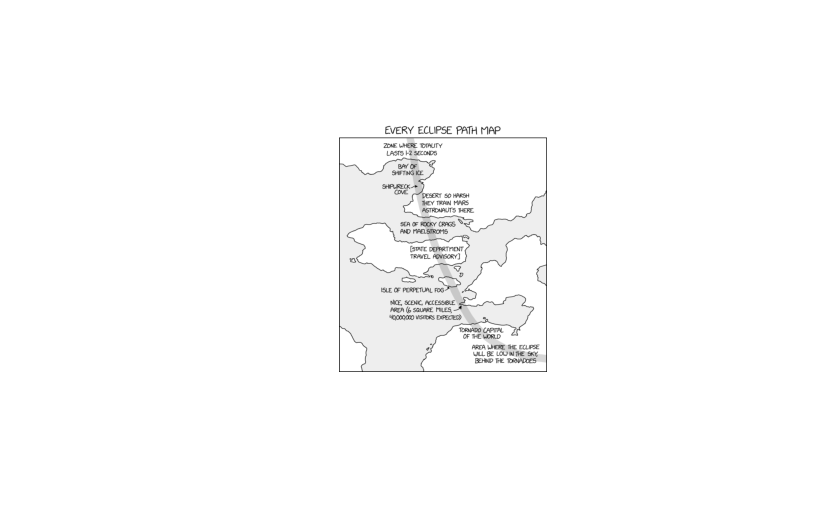
\includegraphics{Part1_Lecture1_Ex_files/figure-pdf/fig-fav-comic-strip-1.pdf}

  }

  \caption{\label{fig-fav-comic-strip}Image of favorite XKCD comic
  strip}

  \end{figure}
\end{enumerate}

\hypertarget{data-viz-with-ggplot2-and-plotly}{%
\subsection{1.2 Data Viz with ggplot2 and
plotly}\label{data-viz-with-ggplot2-and-plotly}}

\hypertarget{exercise-1.2.-data-viz-with-ggplot2-and-plotly}{%
\subsubsection{Exercise 1.2. Data Viz with ggplot2 and
plotly}\label{exercise-1.2.-data-viz-with-ggplot2-and-plotly}}

\hypertarget{exercise-1.2-task-1-create-a-basic-scatterplot}{%
\paragraph{Exercise 1.2 -- Task 1: Create a basic
Scatterplot}\label{exercise-1.2-task-1-create-a-basic-scatterplot}}

Install and load the libraries ``tidyverse'', ``ggplot2'', ``plotly''
and ``palmerpenguins''.

View the data using View(penguins).

Read the help page of the penguins dataset using help(penguins). It
contains a data dictionary explaining attribute semantics.

Type glimpse(penguins) and summary(penguins) and inspect the output.

\begin{itemize}
\item
  glimpse() shows you all the attributes, their data types and some
  example values. glimpse() is part of the dyplyr package, which in turn
  is part of the tidyverse collection of packages.
\item
  summary() is a generic function. Applied to a data set, it shows you
  summary statistics of all attributes.
\end{itemize}

Plot all pairs of variables against each other using ggpairs().

\begin{figure}

{\centering \includegraphics[width=3.64583in,height=\textheight]{Materials L1/Exercise 1.2 – Task 1 Create a basic Scatterplot.PNG}

}

\caption{\label{fig-desired-scatterplot}Desired Scatterplot}

\end{figure}

Recreate the scatterplot on the right (see
Figure~\ref{fig-desired-scatterplot} and for solution
Figure~\ref{fig-penguins-ggpairs-1} and
Figure~\ref{fig-penguins-ggpairs-2}):

\begin{itemize}
\item
  Start with an empty canvas using ggplot() and specify the data set.
\item
  Then add an aestetic mapping using mapping() and aes().
\item
  In aes(), map flipper\_length\_mm to the x-axes and bill\_length\_mm
  to the y axes.
\item
  Add a layer geom\_point() to visualize the corresponding data as a
  scatterplot.
\end{itemize}

\begin{Shaded}
\begin{Highlighting}[]
\CommentTok{\# install.packages("tidyverse") \# already installed}
\CommentTok{\# install.packages("ggplot2") \# already installed}
\CommentTok{\# install.packages("plotly") \# already installed}
\CommentTok{\# install.packages("palmerpenguins") \# already installed}

\CommentTok{\# install.packages("GGally") \# already isntalled \# needed for the ggpairs()}
\FunctionTok{library}\NormalTok{(}\StringTok{"GGally"}\NormalTok{) }\CommentTok{\# needed for the ggpairs()}

\FunctionTok{library}\NormalTok{(}\StringTok{"tidyverse"}\NormalTok{)}
\FunctionTok{library}\NormalTok{(}\StringTok{"ggplot2"}\NormalTok{)}
\FunctionTok{library}\NormalTok{(}\StringTok{"plotly"}\NormalTok{)}
\FunctionTok{library}\NormalTok{(}\StringTok{"palmerpenguins"}\NormalTok{)}

\FunctionTok{View}\NormalTok{(penguins)}

\FunctionTok{help}\NormalTok{(}\StringTok{"penguins"}\NormalTok{)}

\FunctionTok{glimpse}\NormalTok{(penguins)}
\end{Highlighting}
\end{Shaded}

\begin{verbatim}
Rows: 344
Columns: 8
$ species           <fct> Adelie, Adelie, Adelie, Adelie, Adelie, Adelie, Adel~
$ island            <fct> Torgersen, Torgersen, Torgersen, Torgersen, Torgerse~
$ bill_length_mm    <dbl> 39.1, 39.5, 40.3, NA, 36.7, 39.3, 38.9, 39.2, 34.1, ~
$ bill_depth_mm     <dbl> 18.7, 17.4, 18.0, NA, 19.3, 20.6, 17.8, 19.6, 18.1, ~
$ flipper_length_mm <int> 181, 186, 195, NA, 193, 190, 181, 195, 193, 190, 186~
$ body_mass_g       <int> 3750, 3800, 3250, NA, 3450, 3650, 3625, 4675, 3475, ~
$ sex               <fct> male, female, female, NA, female, male, female, male~
$ year              <int> 2007, 2007, 2007, 2007, 2007, 2007, 2007, 2007, 2007~
\end{verbatim}

\begin{Shaded}
\begin{Highlighting}[]
\FunctionTok{summary}\NormalTok{(penguins)}
\end{Highlighting}
\end{Shaded}

\begin{verbatim}
      species          island    bill_length_mm  bill_depth_mm  
 Adelie   :152   Biscoe   :168   Min.   :32.10   Min.   :13.10  
 Chinstrap: 68   Dream    :124   1st Qu.:39.23   1st Qu.:15.60  
 Gentoo   :124   Torgersen: 52   Median :44.45   Median :17.30  
                                 Mean   :43.92   Mean   :17.15  
                                 3rd Qu.:48.50   3rd Qu.:18.70  
                                 Max.   :59.60   Max.   :21.50  
                                 NA's   :2       NA's   :2      
 flipper_length_mm  body_mass_g       sex           year     
 Min.   :172.0     Min.   :2700   female:165   Min.   :2007  
 1st Qu.:190.0     1st Qu.:3550   male  :168   1st Qu.:2007  
 Median :197.0     Median :4050   NA's  : 11   Median :2008  
 Mean   :200.9     Mean   :4202                Mean   :2008  
 3rd Qu.:213.0     3rd Qu.:4750                3rd Qu.:2009  
 Max.   :231.0     Max.   :6300                Max.   :2009  
 NA's   :2         NA's   :2                                 
\end{verbatim}

\begin{Shaded}
\begin{Highlighting}[]
\FunctionTok{ggpairs}\NormalTok{(penguins) }


\FunctionTok{ggplot}\NormalTok{(}\AttributeTok{data =}\NormalTok{ penguins,}
       \AttributeTok{mapping =} \FunctionTok{aes}\NormalTok{(}\AttributeTok{x =}\NormalTok{ flipper\_length\_mm, }
                     \AttributeTok{y =}\NormalTok{ bill\_length\_mm)) }\SpecialCharTok{+} 
  \FunctionTok{geom\_point}\NormalTok{()}
\end{Highlighting}
\end{Shaded}

\begin{figure}

\begin{minipage}[t]{0.50\linewidth}

{\centering 

\raisebox{-\height}{

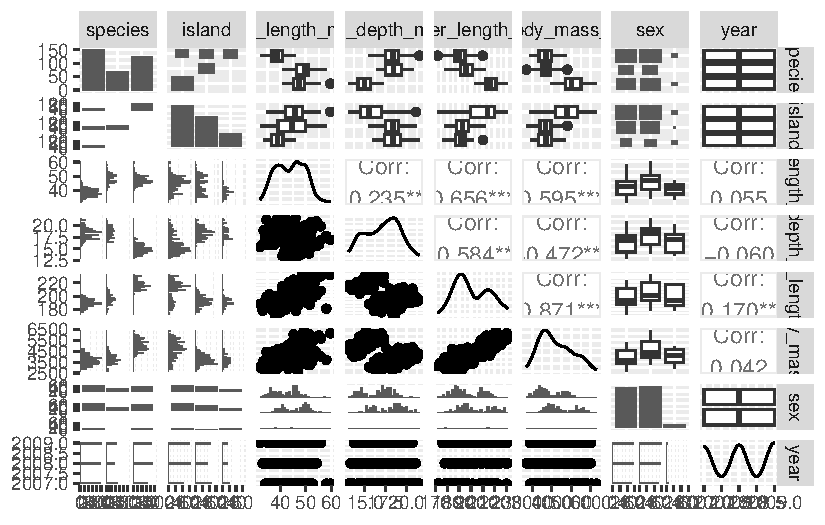
\includegraphics{Part1_Lecture1_Ex_files/figure-pdf/fig-penguins-ggpairs-1.pdf}

}

}

\subcaption{\label{fig-penguins-ggpairs-1}Penguins ggpairs}
\end{minipage}%
%
\begin{minipage}[t]{0.50\linewidth}

{\centering 

\raisebox{-\height}{

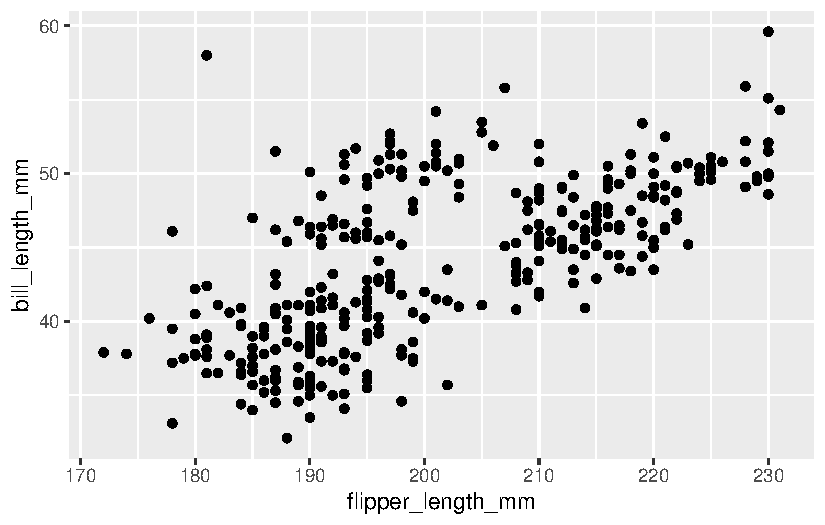
\includegraphics{Part1_Lecture1_Ex_files/figure-pdf/fig-penguins-ggpairs-2.pdf}

}

}

\subcaption{\label{fig-penguins-ggpairs-2}Penguins Scatterplot}
\end{minipage}%

\caption{\label{fig-penguins-ggpairs}Penguins}

\end{figure}

\hypertarget{exercise-1.2-task-2-pimp-up-your-scatterplot}{%
\paragraph{Exercise 1.2 -- Task 2: Pimp Up your
Scatterplot}\label{exercise-1.2-task-2-pimp-up-your-scatterplot}}

\begin{figure}

{\centering \includegraphics[width=3.64583in,height=\textheight]{Materials L1/Exercise 1.2 – Task 2 Pimp Up your Scatterplot.PNG}

}

\caption{\label{fig-desired-scatterplot2}Desired Scatterplot (pimed)}

\end{figure}

Add the variable island to your plot by mapping it to the color channel.

Add another layer labs() to your plot and use it to add the title
``Flipper Length vs.~Bill Length (in mm) by Island''. To see all
arguments of the labs() function, type help(labs).

Use labs() to add the subtitle ``Source: Palmer Station LTER /
palmerpenguins package''

Use labs() to change the labels of the x and y axes to ``Flipper Length
(mm)'' and ``Bill Length (mm)'', respectively.

Use labs() to change the legend title to ``Island''.

Now your plot should look like the one on the right! (see
Figure~\ref{fig-desired-scatterplot2} and for solution
Figure~\ref{fig-penguins-pimped-scatterplot})

\begin{Shaded}
\begin{Highlighting}[]
\CommentTok{\# install.packages("tidyverse") \# already installed}
\CommentTok{\# install.packages("ggplot2") \# already installed}
\CommentTok{\# install.packages("plotly") \# already installed}
\CommentTok{\# install.packages("palmerpenguins") \# already installed}
\FunctionTok{library}\NormalTok{(}\StringTok{"tidyverse"}\NormalTok{)}
\FunctionTok{library}\NormalTok{(}\StringTok{"ggplot2"}\NormalTok{)}
\FunctionTok{library}\NormalTok{(}\StringTok{"plotly"}\NormalTok{)}
\FunctionTok{library}\NormalTok{(}\StringTok{"palmerpenguins"}\NormalTok{)}

\FunctionTok{ggplot}\NormalTok{(}\AttributeTok{data =}\NormalTok{ penguins,}
       \AttributeTok{mapping =} \FunctionTok{aes}\NormalTok{(}\AttributeTok{x =}\NormalTok{ flipper\_length\_mm, }
                     \AttributeTok{y =}\NormalTok{ bill\_length\_mm, }
                     \AttributeTok{color =}\NormalTok{ island)) }\SpecialCharTok{+} 
  \FunctionTok{geom\_point}\NormalTok{() }\SpecialCharTok{+}
  \FunctionTok{labs}\NormalTok{(}\AttributeTok{title =} \StringTok{"Flipper Length vs. Bill Length (in mm) by Island"}\NormalTok{,}
       \AttributeTok{subtitle =} \StringTok{"Source: Palmer Station LTER / palmerpenguins package"}\NormalTok{,}
          \AttributeTok{x =} \StringTok{"Flipper Length (mm)"}\NormalTok{, }\AttributeTok{y =} \StringTok{"Bill Length (mm)"}\NormalTok{,}
       \AttributeTok{color =} \StringTok{"Island"}\NormalTok{) }\CommentTok{\# Set legend title for color scale }
\end{Highlighting}
\end{Shaded}

\begin{figure}[H]

{\centering 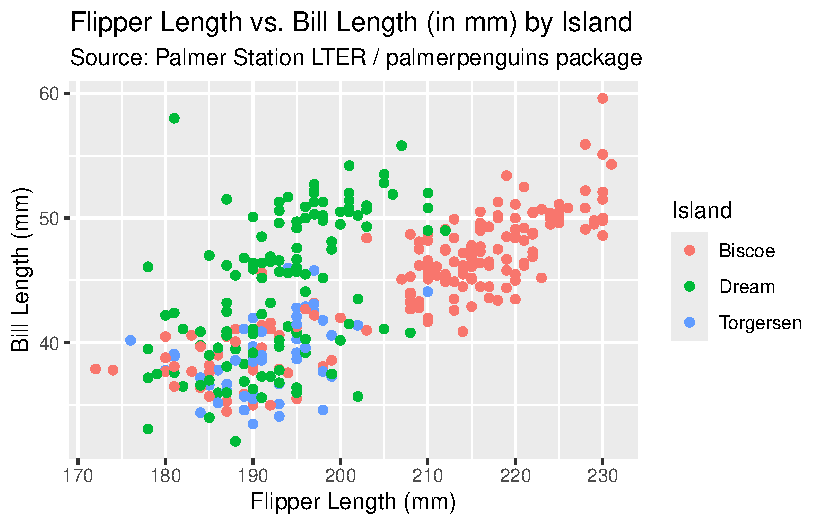
\includegraphics{Part1_Lecture1_Ex_files/figure-pdf/fig-penguins-pimped-scatterplot-1.pdf}

}

\caption{\label{fig-penguins-pimped-scatterplot}Penguins pimped
Scatterplot}

\end{figure}

\hypertarget{exercise-1.2-task-3-add-a-smoothed-trendline}{%
\paragraph{Exercise 1.2 -- Task 3: Add a Smoothed
Trendline}\label{exercise-1.2-task-3-add-a-smoothed-trendline}}

\begin{figure}

{\centering \includegraphics[width=3.64583in,height=\textheight]{Materials L1/Exercise 1.2 – Task 3 Add a Smoothed Trendline.PNG}

}

\caption{\label{fig-scatterplot-trendline}Desired Scatterplot with
trendline}

\end{figure}

Now add a layer geom\_smooth to visualize a smoothed trendline. What
happens here?

\begin{itemize}
\tightlist
\item
  Answer: 3 trendlines get shown, as the variables island is mapped to
  the color scale
\end{itemize}

Change your plot so that only one trendline is displayed.

Make it interactive using ggplotly().

\begin{itemize}
\tightlist
\item
  Remark: To do that, assign your whole plot from (b) to a variable,
  e.g., the variable my\_plot. Then call ggploty(my\_plot).
\end{itemize}

Now your plot should look like the one on the right! (see
Figure~\ref{fig-scatterplot-trendline} and for solution
Figure~\ref{fig-penguins-scatterplot-trendline})

\begin{Shaded}
\begin{Highlighting}[]
\CommentTok{\# install.packages("tidyverse") \# already installed}
\CommentTok{\# install.packages("ggplot2") \# already installed}
\CommentTok{\# install.packages("plotly") \# already installed}
\CommentTok{\# install.packages("palmerpenguins") \# already installed}
\FunctionTok{library}\NormalTok{(}\StringTok{"tidyverse"}\NormalTok{)}
\FunctionTok{library}\NormalTok{(}\StringTok{"ggplot2"}\NormalTok{)}
\FunctionTok{library}\NormalTok{(}\StringTok{"plotly"}\NormalTok{)}
\FunctionTok{library}\NormalTok{(}\StringTok{"palmerpenguins"}\NormalTok{)}

\NormalTok{my\_plot }\OtherTok{\textless{}{-}} \FunctionTok{ggplot}\NormalTok{(}\AttributeTok{data =}\NormalTok{ penguins,}
                  \AttributeTok{mapping =} \FunctionTok{aes}\NormalTok{(}\AttributeTok{x =}\NormalTok{ flipper\_length\_mm, }
                                \AttributeTok{y =}\NormalTok{ bill\_length\_mm)) }\SpecialCharTok{+} 
  \FunctionTok{geom\_point}\NormalTok{(}\AttributeTok{mapping =} \FunctionTok{aes}\NormalTok{(}\AttributeTok{color =}\NormalTok{ island)) }\SpecialCharTok{+} \CommentTok{\# mapping for the color scale to the "point", so only one trendline appears}
  \FunctionTok{geom\_smooth}\NormalTok{() }\SpecialCharTok{+}
  \FunctionTok{labs}\NormalTok{(}\AttributeTok{title =} \StringTok{"Flipper Length vs. Bill Length (in mm) by Island"}\NormalTok{,}
       \AttributeTok{subtitle =} \StringTok{"Source: Palmer Station LTER / palmerpenguins package"}\NormalTok{,}
       \AttributeTok{x =} \StringTok{"Flipper Length (mm)"}\NormalTok{, }\AttributeTok{y =} \StringTok{"Bill Length (mm)"}\NormalTok{,}
       \AttributeTok{color =} \StringTok{"Island"}\NormalTok{) }\CommentTok{\# Set legend title for color scale}

\FunctionTok{ggplotly}\NormalTok{(my\_plot)}
\end{Highlighting}
\end{Shaded}

\begin{figure}

{\centering 

}

\caption{\label{fig-penguins-scatterplot-trendline}Penguins Scatterplot
with trendline}

\end{figure}

\hypertarget{exercise-1.2-task-4-create-a-stacked-bar-plot}{%
\paragraph{Exercise 1.2 -- Task 4: Create a Stacked Bar
Plot}\label{exercise-1.2-task-4-create-a-stacked-bar-plot}}

\begin{figure}

{\centering \includegraphics[width=3.64583in,height=\textheight]{Materials L1/Exercise 1.2 – Task 4 Create a Stacked Bar Plot.PNG}

}

\caption{\label{fig-desired-output-canvas}Desired Output}

\end{figure}

Create a new canvas for penguins.

Create a bar plot of the variable species using geom\_bar.

Use facet\_wrap() to create a sequence of facets along the variable
island.

In facet\_wrap(), add the argument ncol=1. (See help(facet\_wrap) for
more arguments!)

In aes(), add the position argument fill = sex. This gives you stacked
bar plots according tp sex.

\begin{itemize}
\tightlist
\item
  Remark: A position adjustment for a geometry (like geom\_bar here)
  specifies a ``rule'' as to how different components should be
  positioned relative to each other to make sure they don't overlap.
  This position adjustment is inherent in geom\_bar, and we can make it
  visible by mapping a different variable to the color encoding (using
  the fill aesthetic here).
\end{itemize}

Now your plot should look like the one on the right! (see
Figure~\ref{fig-desired-output-canvas} and for solution
Figure~\ref{fig-penguins-barchart})

\begin{Shaded}
\begin{Highlighting}[]
\FunctionTok{ggplot}\NormalTok{(}\AttributeTok{data=}\NormalTok{penguins) }\SpecialCharTok{+} 
  \FunctionTok{geom\_bar}\NormalTok{(}\AttributeTok{mapping =} \FunctionTok{aes}\NormalTok{(}\AttributeTok{x=}\NormalTok{species, }\AttributeTok{fill=}\NormalTok{sex)) }\SpecialCharTok{+}
  \FunctionTok{facet\_wrap}\NormalTok{(}\AttributeTok{facets=}\SpecialCharTok{\textasciitilde{}}\NormalTok{island,}
             \AttributeTok{ncol=}\DecValTok{1}\NormalTok{)}
\end{Highlighting}
\end{Shaded}

\begin{figure}[H]

{\centering 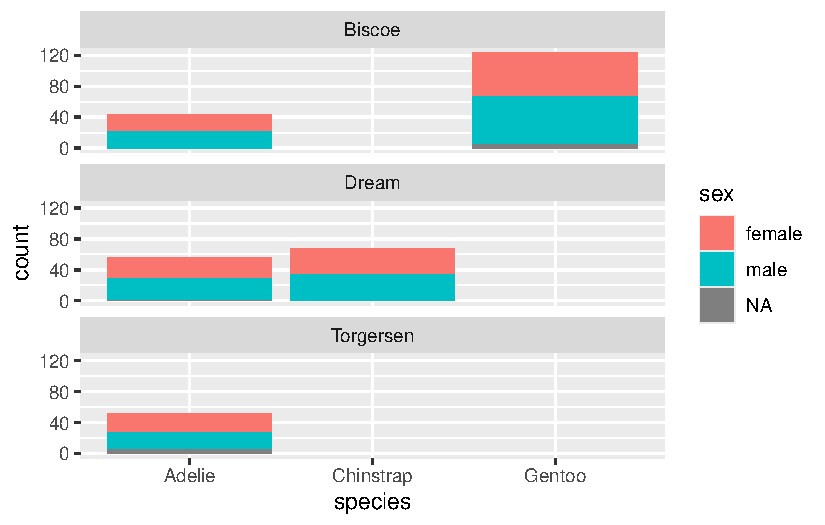
\includegraphics{Part1_Lecture1_Ex_files/figure-pdf/fig-penguins-barchart-1.pdf}

}

\caption{\label{fig-penguins-barchart}Penguins Barchart per islands}

\end{figure}

\hypertarget{self-study-1.2.-data-viz-with-ggplot2-and-plotly}{%
\subsubsection{Self-Study 1.2. Data Viz with ggplot2 and
plotly}\label{self-study-1.2.-data-viz-with-ggplot2-and-plotly}}

\hypertarget{self-study-1.2-task-1-business-understanding}{%
\paragraph{Self Study 1.2 -- Task 1: Business
Understanding}\label{self-study-1.2-task-1-business-understanding}}

\begin{enumerate}
\def\labelenumi{\arabic{enumi}.}
\item
  Install and load the libraries ``tidyverse'', ``ggplot2'', ``plotly'',
  ``skimr'' and ``Ggally''
\item
  The data set mpg is included in the ggplot2 package. Read the help
  page of the dataset using help(mpg). It contains a data dictionary.
\item
  Try to understand what the attribute names mean.
\item
  View the data using View(mpg).
\end{enumerate}

\begin{Shaded}
\begin{Highlighting}[]
\CommentTok{\# install.packages("tidyverse") \# already installed}
\CommentTok{\# install.packages("ggplot2") \# already installed}
\CommentTok{\# install.packages("plotly") \# already installed}
\CommentTok{\# install.packages("skimr") \# already installed}
\CommentTok{\# install.packages("GGally") \# already installed}

\FunctionTok{library}\NormalTok{(}\StringTok{"tidyverse"}\NormalTok{)}
\FunctionTok{library}\NormalTok{(}\StringTok{"ggplot2"}\NormalTok{)}
\FunctionTok{library}\NormalTok{(}\StringTok{"plotly"}\NormalTok{)}
\FunctionTok{library}\NormalTok{(}\StringTok{"skimr"}\NormalTok{)}
\FunctionTok{library}\NormalTok{(}\StringTok{"GGally"}\NormalTok{)}

\FunctionTok{help}\NormalTok{(mpg)}

\FunctionTok{View}\NormalTok{(mpg)}
\end{Highlighting}
\end{Shaded}

\hypertarget{self-study-1.2-task-2-data-understanding-based-on-summary-statistics}{%
\paragraph{Self Study 1.2 -- Task 2: Data Understanding based on Summary
Statistics}\label{self-study-1.2-task-2-data-understanding-based-on-summary-statistics}}

Use the functions class(), typeof(), attributes() and dim() to check the
class, data type, attributes and dimensions of the mpg dataset. Notice
that mpg is loaded as a table (tbl) - a special kind of data frame (see
later).

Get a first impression of the structure of the data by calling
glimpse(mpg) and summary(mpg)

Now try the skim() function from the skimr library to get a better
overview over the dataset. Look into the help page of skim(). (see
Figure~\ref{fig-mpg-skim} for the output)

Now answer the following questions:

\begin{itemize}
\item
  Data of how many cars are stored in the data set?

  \emph{Solution: 234 (number of rows)}
\item
  How many car attributes have been recorded in the mpg data set?

  \emph{Solution: 11 (number of columns)}
\item
  How many of them are numerical, how many categorical?

  \emph{Solution: 5 numeric (numerical) and 6 character (categorical)}
\item
  Has the attribute type of drive train been recorded for all cars in
  this data set, or are there any missing values for this attribute?

  \emph{Solution: there are 0 missing values}
\item
  How many car models does this data set contain?

  \emph{Solution: there are 38 car models (n\_unique)}
\item
  How many manufacturers?

  \emph{Solution: there are 15 manufacturers (n\_unique)}
\end{itemize}

\begin{Shaded}
\begin{Highlighting}[]
\FunctionTok{class}\NormalTok{(mpg)}
\end{Highlighting}
\end{Shaded}

\begin{verbatim}
[1] "tbl_df"     "tbl"        "data.frame"
\end{verbatim}

\begin{Shaded}
\begin{Highlighting}[]
\FunctionTok{typeof}\NormalTok{(mpg)}
\end{Highlighting}
\end{Shaded}

\begin{verbatim}
[1] "list"
\end{verbatim}

\begin{Shaded}
\begin{Highlighting}[]
\FunctionTok{attributes}\NormalTok{(mpg) }\CommentTok{\# gives: class, row.names, names(headers)}
\end{Highlighting}
\end{Shaded}

\begin{verbatim}
$class
[1] "tbl_df"     "tbl"        "data.frame"

$row.names
  [1]   1   2   3   4   5   6   7   8   9  10  11  12  13  14  15  16  17  18
 [19]  19  20  21  22  23  24  25  26  27  28  29  30  31  32  33  34  35  36
 [37]  37  38  39  40  41  42  43  44  45  46  47  48  49  50  51  52  53  54
 [55]  55  56  57  58  59  60  61  62  63  64  65  66  67  68  69  70  71  72
 [73]  73  74  75  76  77  78  79  80  81  82  83  84  85  86  87  88  89  90
 [91]  91  92  93  94  95  96  97  98  99 100 101 102 103 104 105 106 107 108
[109] 109 110 111 112 113 114 115 116 117 118 119 120 121 122 123 124 125 126
[127] 127 128 129 130 131 132 133 134 135 136 137 138 139 140 141 142 143 144
[145] 145 146 147 148 149 150 151 152 153 154 155 156 157 158 159 160 161 162
[163] 163 164 165 166 167 168 169 170 171 172 173 174 175 176 177 178 179 180
[181] 181 182 183 184 185 186 187 188 189 190 191 192 193 194 195 196 197 198
[199] 199 200 201 202 203 204 205 206 207 208 209 210 211 212 213 214 215 216
[217] 217 218 219 220 221 222 223 224 225 226 227 228 229 230 231 232 233 234

$names
 [1] "manufacturer" "model"        "displ"        "year"         "cyl"         
 [6] "trans"        "drv"          "cty"          "hwy"          "fl"          
[11] "class"       
\end{verbatim}

\begin{Shaded}
\begin{Highlighting}[]
\FunctionTok{dim}\NormalTok{(mpg) }\CommentTok{\# dimension: rows x columns}
\end{Highlighting}
\end{Shaded}

\begin{verbatim}
[1] 234  11
\end{verbatim}

\begin{Shaded}
\begin{Highlighting}[]
\FunctionTok{glimpse}\NormalTok{(mpg) }
\end{Highlighting}
\end{Shaded}

\begin{verbatim}
Rows: 234
Columns: 11
$ manufacturer <chr> "audi", "audi", "audi", "audi", "audi", "audi", "audi", "~
$ model        <chr> "a4", "a4", "a4", "a4", "a4", "a4", "a4", "a4 quattro", "~
$ displ        <dbl> 1.8, 1.8, 2.0, 2.0, 2.8, 2.8, 3.1, 1.8, 1.8, 2.0, 2.0, 2.~
$ year         <int> 1999, 1999, 2008, 2008, 1999, 1999, 2008, 1999, 1999, 200~
$ cyl          <int> 4, 4, 4, 4, 6, 6, 6, 4, 4, 4, 4, 6, 6, 6, 6, 6, 6, 8, 8, ~
$ trans        <chr> "auto(l5)", "manual(m5)", "manual(m6)", "auto(av)", "auto~
$ drv          <chr> "f", "f", "f", "f", "f", "f", "f", "4", "4", "4", "4", "4~
$ cty          <int> 18, 21, 20, 21, 16, 18, 18, 18, 16, 20, 19, 15, 17, 17, 1~
$ hwy          <int> 29, 29, 31, 30, 26, 26, 27, 26, 25, 28, 27, 25, 25, 25, 2~
$ fl           <chr> "p", "p", "p", "p", "p", "p", "p", "p", "p", "p", "p", "p~
$ class        <chr> "compact", "compact", "compact", "compact", "compact", "c~
\end{verbatim}

\begin{Shaded}
\begin{Highlighting}[]
\FunctionTok{summary}\NormalTok{(mpg)}
\end{Highlighting}
\end{Shaded}

\begin{verbatim}
 manufacturer          model               displ            year     
 Length:234         Length:234         Min.   :1.600   Min.   :1999  
 Class :character   Class :character   1st Qu.:2.400   1st Qu.:1999  
 Mode  :character   Mode  :character   Median :3.300   Median :2004  
                                       Mean   :3.472   Mean   :2004  
                                       3rd Qu.:4.600   3rd Qu.:2008  
                                       Max.   :7.000   Max.   :2008  
      cyl           trans               drv                 cty       
 Min.   :4.000   Length:234         Length:234         Min.   : 9.00  
 1st Qu.:4.000   Class :character   Class :character   1st Qu.:14.00  
 Median :6.000   Mode  :character   Mode  :character   Median :17.00  
 Mean   :5.889                                         Mean   :16.86  
 3rd Qu.:8.000                                         3rd Qu.:19.00  
 Max.   :8.000                                         Max.   :35.00  
      hwy             fl               class          
 Min.   :12.00   Length:234         Length:234        
 1st Qu.:18.00   Class :character   Class :character  
 Median :24.00   Mode  :character   Mode  :character  
 Mean   :23.44                                        
 3rd Qu.:27.00                                        
 Max.   :44.00                                        
\end{verbatim}

\begin{Shaded}
\begin{Highlighting}[]
\FunctionTok{skim}\NormalTok{(mpg)}
\end{Highlighting}
\end{Shaded}

\begin{longtable}[]{@{}ll@{}}
\caption{Data summary}\tabularnewline
\toprule\noalign{}
\endfirsthead
\endhead
\bottomrule\noalign{}
\endlastfoot
Name & mpg \\
Number of rows & 234 \\
Number of columns & 11 \\
\_\_\_\_\_\_\_\_\_\_\_\_\_\_\_\_\_\_\_\_\_\_\_ & \\
Column type frequency: & \\
character & 6 \\
numeric & 5 \\
\_\_\_\_\_\_\_\_\_\_\_\_\_\_\_\_\_\_\_\_\_\_\_\_ & \\
Group variables & None \\
\end{longtable}

\textbf{Variable type: character}

\begin{longtable}[]{@{}
  >{\raggedright\arraybackslash}p{(\columnwidth - 14\tabcolsep) * \real{0.1944}}
  >{\raggedleft\arraybackslash}p{(\columnwidth - 14\tabcolsep) * \real{0.1389}}
  >{\raggedleft\arraybackslash}p{(\columnwidth - 14\tabcolsep) * \real{0.1944}}
  >{\raggedleft\arraybackslash}p{(\columnwidth - 14\tabcolsep) * \real{0.0556}}
  >{\raggedleft\arraybackslash}p{(\columnwidth - 14\tabcolsep) * \real{0.0556}}
  >{\raggedleft\arraybackslash}p{(\columnwidth - 14\tabcolsep) * \real{0.0833}}
  >{\raggedleft\arraybackslash}p{(\columnwidth - 14\tabcolsep) * \real{0.1250}}
  >{\raggedleft\arraybackslash}p{(\columnwidth - 14\tabcolsep) * \real{0.1528}}@{}}
\toprule\noalign{}
\begin{minipage}[b]{\linewidth}\raggedright
skim\_variable
\end{minipage} & \begin{minipage}[b]{\linewidth}\raggedleft
n\_missing
\end{minipage} & \begin{minipage}[b]{\linewidth}\raggedleft
complete\_rate
\end{minipage} & \begin{minipage}[b]{\linewidth}\raggedleft
min
\end{minipage} & \begin{minipage}[b]{\linewidth}\raggedleft
max
\end{minipage} & \begin{minipage}[b]{\linewidth}\raggedleft
empty
\end{minipage} & \begin{minipage}[b]{\linewidth}\raggedleft
n\_unique
\end{minipage} & \begin{minipage}[b]{\linewidth}\raggedleft
whitespace
\end{minipage} \\
\midrule\noalign{}
\endhead
\bottomrule\noalign{}
\endlastfoot
manufacturer & 0 & 1 & 4 & 10 & 0 & 15 & 0 \\
model & 0 & 1 & 2 & 22 & 0 & 38 & 0 \\
trans & 0 & 1 & 8 & 10 & 0 & 10 & 0 \\
drv & 0 & 1 & 1 & 1 & 0 & 3 & 0 \\
fl & 0 & 1 & 1 & 1 & 0 & 5 & 0 \\
class & 0 & 1 & 3 & 10 & 0 & 7 & 0 \\
\end{longtable}

\textbf{Variable type: numeric}

\begin{longtable}[]{@{}
  >{\raggedright\arraybackslash}p{(\columnwidth - 20\tabcolsep) * \real{0.1556}}
  >{\raggedleft\arraybackslash}p{(\columnwidth - 20\tabcolsep) * \real{0.1111}}
  >{\raggedleft\arraybackslash}p{(\columnwidth - 20\tabcolsep) * \real{0.1556}}
  >{\raggedleft\arraybackslash}p{(\columnwidth - 20\tabcolsep) * \real{0.0889}}
  >{\raggedleft\arraybackslash}p{(\columnwidth - 20\tabcolsep) * \real{0.0556}}
  >{\raggedleft\arraybackslash}p{(\columnwidth - 20\tabcolsep) * \real{0.0778}}
  >{\raggedleft\arraybackslash}p{(\columnwidth - 20\tabcolsep) * \real{0.0778}}
  >{\raggedleft\arraybackslash}p{(\columnwidth - 20\tabcolsep) * \real{0.0778}}
  >{\raggedleft\arraybackslash}p{(\columnwidth - 20\tabcolsep) * \real{0.0778}}
  >{\raggedleft\arraybackslash}p{(\columnwidth - 20\tabcolsep) * \real{0.0556}}
  >{\raggedright\arraybackslash}p{(\columnwidth - 20\tabcolsep) * \real{0.0667}}@{}}
\toprule\noalign{}
\begin{minipage}[b]{\linewidth}\raggedright
skim\_variable
\end{minipage} & \begin{minipage}[b]{\linewidth}\raggedleft
n\_missing
\end{minipage} & \begin{minipage}[b]{\linewidth}\raggedleft
complete\_rate
\end{minipage} & \begin{minipage}[b]{\linewidth}\raggedleft
mean
\end{minipage} & \begin{minipage}[b]{\linewidth}\raggedleft
sd
\end{minipage} & \begin{minipage}[b]{\linewidth}\raggedleft
p0
\end{minipage} & \begin{minipage}[b]{\linewidth}\raggedleft
p25
\end{minipage} & \begin{minipage}[b]{\linewidth}\raggedleft
p50
\end{minipage} & \begin{minipage}[b]{\linewidth}\raggedleft
p75
\end{minipage} & \begin{minipage}[b]{\linewidth}\raggedleft
p100
\end{minipage} & \begin{minipage}[b]{\linewidth}\raggedright
hist
\end{minipage} \\
\midrule\noalign{}
\endhead
\bottomrule\noalign{}
\endlastfoot
displ & 0 & 1 & 3.47 & 1.29 & 1.6 & 2.4 & 3.3 & 4.6 & 7 & ▇▆▆▃▁ \\
year & 0 & 1 & 2003.50 & 4.51 & 1999.0 & 1999.0 & 2003.5 & 2008.0 & 2008
& ▇▁▁▁▇ \\
cyl & 0 & 1 & 5.89 & 1.61 & 4.0 & 4.0 & 6.0 & 8.0 & 8 & ▇▁▇▁▇ \\
cty & 0 & 1 & 16.86 & 4.26 & 9.0 & 14.0 & 17.0 & 19.0 & 35 & ▆▇▃▁▁ \\
hwy & 0 & 1 & 23.44 & 5.95 & 12.0 & 18.0 & 24.0 & 27.0 & 44 & ▅▅▇▁▁ \\
\end{longtable}

\begin{itemize}
\item
  What is the minimum number of cylinders that occur in a car of this
  data set?

  \emph{Solution: 4 (in skim the min appears under ``p0'' - the zero
  percentile)}
\item
  What is the range of highway miles per gallon of the cars in this data
  set? (range = max-min)

  \emph{Solution: 12 - 44 = 32 (p0 - p100)}
\item
  What is the mean and standard deviation of highway miles per gallon of
  the cars in this data set?

  \emph{Solution: mean= 23.44, sd =5.95}
\item
  In the character variables section, what do you think do the column
  names min, max and empty stand for?

  \begin{itemize}
  \tightlist
  \item
    Hint: Execute unique(mpg\$manufacturer). Does it give you an idea?
  \end{itemize}

  \emph{Solution: \textbf{min = 4} is the minimum number of characters
  of any manufacturer (audi, ford, jeep), \textbf{max = 10} is the
  maximum number of characters of any manufacturer (volkswagen, land
  rover), \textbf{empty = 0} says that no character strings are empty}
\item
  Is the variable cty normally distributed? Is it skewed? (Read this off
  the output of skim.)

  \emph{Solution: Skewness is a measure of the asymmetry of the
  probability distribution about its mean. The little picture displayed
  by skim() suggests that cty is right skewed, since it shows a long
  tail on the right. Yet, the mean is a bit left of the median (p50). So
  it is not clear from the data we see here}.
\item
  Now plot the histogram of cty to double check the sample distribution.
  Do you think it makes sense to check for outliers?

  \emph{Solution: We see also here no clear picture: The mass of the
  distribution may actually be equally distributed about the mean of
  16.9. The little picture may have given a wrong impression because of
  the 2 outliers on the right. As a next step, we could remove the
  outliers and then check the distribution again. But first lets check
  if these are indeed outliers or not\ldots{} (We will learn in a later
  lecture how to remove them, if necessary.)}
\item
  Create a boxplot of the variable cty. Make your boxplot interactive
  using ggplotly(). How many outliers do you see (according to the
  interquartile range (IQR) criterion)?

  \begin{itemize}
  \item
    Hint: In the boxplot, outliers according to the IQR criterion are
    all points outside of the whiskers. (see
    Figure~\ref{fig-iqr-criterion})

    \begin{figure}

    {\centering 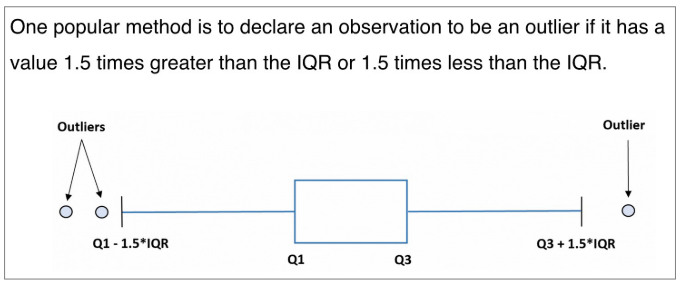
\includegraphics[width=4.6875in,height=\textheight]{Materials L1/IQR criterion.PNG}

    }

    \caption{\label{fig-iqr-criterion}The IQR criterion.}

    \end{figure}
  \end{itemize}

  \emph{Solution: There are 4 outliers visible in the boxplot: The two
  we recognized in the histogram (33 and 35: double check wit the
  histogram), and 2 more (28 and 29).}
\item
  You can check if you are right using the function boxplot.stats():
  Executing boxplot.stats(mpg\$cty)\$out will give you all outliers.
  Does it fit? (Remember that the \$ sign lets you access the single
  attributes of a data frame.)

  \emph{Solution: No, it doesnt fit full: We have actually 5 outliers,
  because 28 appears twice. We couldn't see that in the boxplot, since
  they are drawn on top of each other.}
\end{itemize}

\begin{Shaded}
\begin{Highlighting}[]
\FunctionTok{unique}\NormalTok{(mpg}\SpecialCharTok{$}\NormalTok{manufacturer)}
\NormalTok{my\_hist\_cty }\OtherTok{\textless{}{-}} \FunctionTok{ggplot}\NormalTok{(}\AttributeTok{data =}\NormalTok{ mpg) }\SpecialCharTok{+}
  \FunctionTok{geom\_histogram}\NormalTok{(}\AttributeTok{mapping =} \FunctionTok{aes}\NormalTok{(}\AttributeTok{x=}\NormalTok{cty))}
\FunctionTok{ggplotly}\NormalTok{(my\_hist\_cty)}
\end{Highlighting}
\end{Shaded}

\begin{verbatim}
`stat_bin()` using `bins = 30`. Pick better value with `binwidth`.
\end{verbatim}

\begin{Shaded}
\begin{Highlighting}[]
\NormalTok{my\_boxplot\_cty }\OtherTok{\textless{}{-}} \FunctionTok{ggplot}\NormalTok{(}\AttributeTok{data =}\NormalTok{ mpg) }\SpecialCharTok{+}
  \FunctionTok{geom\_boxplot}\NormalTok{(}\AttributeTok{mapping =} \FunctionTok{aes}\NormalTok{(}\AttributeTok{y=}\NormalTok{cty))}
\FunctionTok{ggplotly}\NormalTok{(my\_boxplot\_cty)}
\FunctionTok{boxplot.stats}\NormalTok{(mpg}\SpecialCharTok{$}\NormalTok{cty)}\SpecialCharTok{$}\NormalTok{out}
\end{Highlighting}
\end{Shaded}

\begin{figure}

\begin{minipage}[t]{\linewidth}

{\centering 

\begin{verbatim}
 [1] "audi"       "chevrolet"  "dodge"      "ford"       "honda"     
 [6] "hyundai"    "jeep"       "land rover" "lincoln"    "mercury"   
[11] "nissan"     "pontiac"    "subaru"     "toyota"     "volkswagen"
\end{verbatim}

}

\end{minipage}%
\newline
\begin{minipage}[t]{\linewidth}

{\centering 

}

\subcaption{\label{fig-mpg-skim-1}histogram of cty}
\end{minipage}%
\newline
\begin{minipage}[t]{\linewidth}

{\centering 

}

\subcaption{\label{fig-mpg-skim-2}outliers}
\end{minipage}%
\newline
\begin{minipage}[t]{\linewidth}

{\centering 

\begin{verbatim}
[1] 28 28 33 35 29
\end{verbatim}

}

\end{minipage}%

\caption{\label{fig-mpg-skim}MPG data}

\end{figure}

\hypertarget{self-study-1.2-task-3-data-understanding-by-visual-eda}{%
\paragraph{Self Study 1.2 -- Task 3: Data Understanding by Visual
EDA}\label{self-study-1.2-task-3-data-understanding-by-visual-eda}}

Now let's do a bit of Exploratory Data Analysis (EDA) using ggplot!

I assume that the number of highway miles a car can go per gallon may
depend functionally on the engine displacement of the car (e.g.,
linearly, quadratically,\ldots). Do you think our sample data will
support my hypothesis? Check by visual inspection.

\begin{itemize}
\item
  Hint: For the visual inspection, make a scatterplot of hwy against
  displ.
\item
  Remark: To really check the hypothesis, we would need to do more: We
  could do a statistical hypothesis test, or we could model a functional
  relationship (as part of the modelling phase of the data science
  lifecycle) and evaluate the modelling results. The step of visual
  inspection is a way of scouting if its worth the effort, and to give
  us ideas. :)
\end{itemize}

\emph{Solution: It looks as if the hypothesis is correct. There is a
clear pattern discernible.}

\begin{Shaded}
\begin{Highlighting}[]
\FunctionTok{ggplot}\NormalTok{(}\AttributeTok{data =}\NormalTok{ mpg, }
       \AttributeTok{mapping =} \FunctionTok{aes}\NormalTok{(}\AttributeTok{x =}\NormalTok{ displ, }
                     \AttributeTok{y =}\NormalTok{ hwy)) }\SpecialCharTok{+}
  \FunctionTok{geom\_point}\NormalTok{()}
\end{Highlighting}
\end{Shaded}

\begin{figure}[H]

{\centering 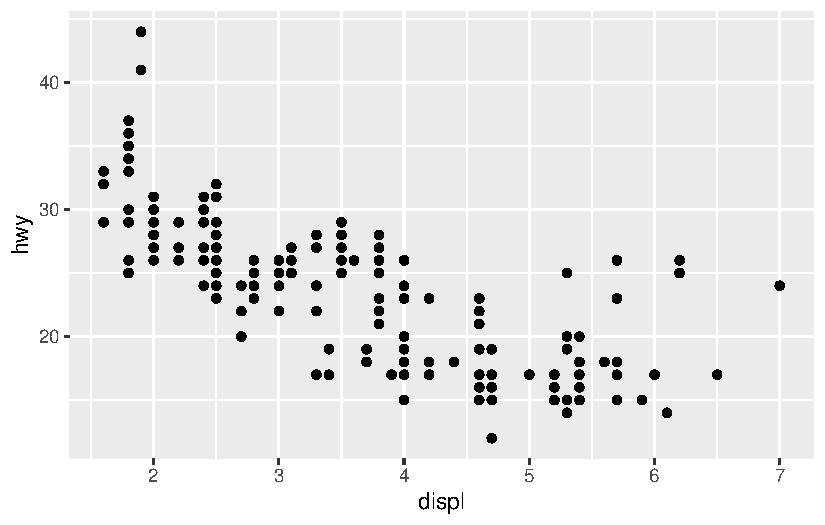
\includegraphics{Part1_Lecture1_Ex_files/figure-pdf/unnamed-chunk-28-1.pdf}

}

\end{figure}

Add the variable year to your plot using color as a third dimension.
What is going on with the legend here?

Solution: The legend shows a continuous scale, even though we actually
only have 2 values of the year variable (1999 and 2008 - check with
unique(mpg\$year)). The reason is that year has been imported as a
numeric data type (check with skim(mpg) or str(mpg)), and this implies a
continuous color scale.

\begin{Shaded}
\begin{Highlighting}[]
\FunctionTok{ggplot}\NormalTok{(}\AttributeTok{data =}\NormalTok{ mpg, }
       \AttributeTok{mapping =} \FunctionTok{aes}\NormalTok{(}\AttributeTok{x =}\NormalTok{ displ, }
                     \AttributeTok{y =}\NormalTok{ hwy,}
                     \AttributeTok{color=}\NormalTok{year)) }\SpecialCharTok{+}
  \FunctionTok{geom\_point}\NormalTok{()}
\end{Highlighting}
\end{Shaded}

\begin{figure}[H]

{\centering 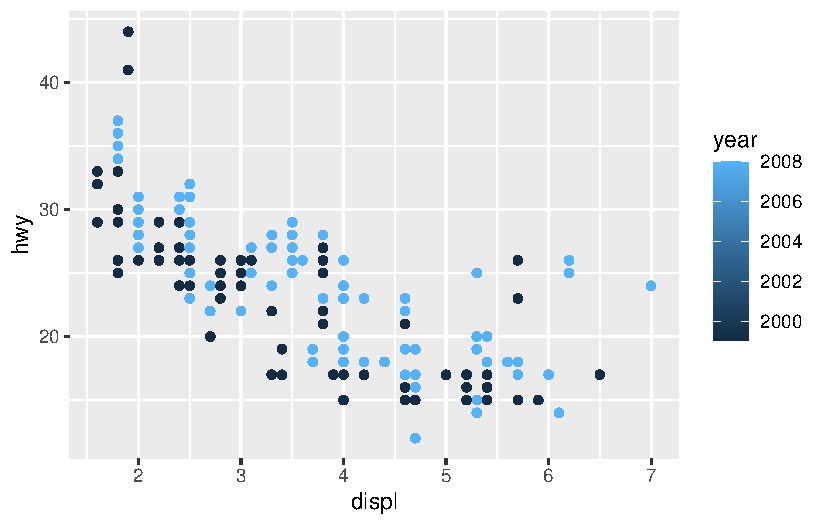
\includegraphics{Part1_Lecture1_Ex_files/figure-pdf/unnamed-chunk-29-1.pdf}

}

\end{figure}

\begin{Shaded}
\begin{Highlighting}[]
\FunctionTok{unique}\NormalTok{(mpg}\SpecialCharTok{$}\NormalTok{year)}
\end{Highlighting}
\end{Shaded}

\begin{verbatim}
[1] 1999 2008
\end{verbatim}

\begin{Shaded}
\begin{Highlighting}[]
\FunctionTok{skim}\NormalTok{(mpg)}
\end{Highlighting}
\end{Shaded}

\begin{longtable}[]{@{}ll@{}}
\caption{Data summary}\tabularnewline
\toprule\noalign{}
\endfirsthead
\endhead
\bottomrule\noalign{}
\endlastfoot
Name & mpg \\
Number of rows & 234 \\
Number of columns & 11 \\
\_\_\_\_\_\_\_\_\_\_\_\_\_\_\_\_\_\_\_\_\_\_\_ & \\
Column type frequency: & \\
character & 6 \\
numeric & 5 \\
\_\_\_\_\_\_\_\_\_\_\_\_\_\_\_\_\_\_\_\_\_\_\_\_ & \\
Group variables & None \\
\end{longtable}

\textbf{Variable type: character}

\begin{longtable}[]{@{}
  >{\raggedright\arraybackslash}p{(\columnwidth - 14\tabcolsep) * \real{0.1944}}
  >{\raggedleft\arraybackslash}p{(\columnwidth - 14\tabcolsep) * \real{0.1389}}
  >{\raggedleft\arraybackslash}p{(\columnwidth - 14\tabcolsep) * \real{0.1944}}
  >{\raggedleft\arraybackslash}p{(\columnwidth - 14\tabcolsep) * \real{0.0556}}
  >{\raggedleft\arraybackslash}p{(\columnwidth - 14\tabcolsep) * \real{0.0556}}
  >{\raggedleft\arraybackslash}p{(\columnwidth - 14\tabcolsep) * \real{0.0833}}
  >{\raggedleft\arraybackslash}p{(\columnwidth - 14\tabcolsep) * \real{0.1250}}
  >{\raggedleft\arraybackslash}p{(\columnwidth - 14\tabcolsep) * \real{0.1528}}@{}}
\toprule\noalign{}
\begin{minipage}[b]{\linewidth}\raggedright
skim\_variable
\end{minipage} & \begin{minipage}[b]{\linewidth}\raggedleft
n\_missing
\end{minipage} & \begin{minipage}[b]{\linewidth}\raggedleft
complete\_rate
\end{minipage} & \begin{minipage}[b]{\linewidth}\raggedleft
min
\end{minipage} & \begin{minipage}[b]{\linewidth}\raggedleft
max
\end{minipage} & \begin{minipage}[b]{\linewidth}\raggedleft
empty
\end{minipage} & \begin{minipage}[b]{\linewidth}\raggedleft
n\_unique
\end{minipage} & \begin{minipage}[b]{\linewidth}\raggedleft
whitespace
\end{minipage} \\
\midrule\noalign{}
\endhead
\bottomrule\noalign{}
\endlastfoot
manufacturer & 0 & 1 & 4 & 10 & 0 & 15 & 0 \\
model & 0 & 1 & 2 & 22 & 0 & 38 & 0 \\
trans & 0 & 1 & 8 & 10 & 0 & 10 & 0 \\
drv & 0 & 1 & 1 & 1 & 0 & 3 & 0 \\
fl & 0 & 1 & 1 & 1 & 0 & 5 & 0 \\
class & 0 & 1 & 3 & 10 & 0 & 7 & 0 \\
\end{longtable}

\textbf{Variable type: numeric}

\begin{longtable}[]{@{}
  >{\raggedright\arraybackslash}p{(\columnwidth - 20\tabcolsep) * \real{0.1556}}
  >{\raggedleft\arraybackslash}p{(\columnwidth - 20\tabcolsep) * \real{0.1111}}
  >{\raggedleft\arraybackslash}p{(\columnwidth - 20\tabcolsep) * \real{0.1556}}
  >{\raggedleft\arraybackslash}p{(\columnwidth - 20\tabcolsep) * \real{0.0889}}
  >{\raggedleft\arraybackslash}p{(\columnwidth - 20\tabcolsep) * \real{0.0556}}
  >{\raggedleft\arraybackslash}p{(\columnwidth - 20\tabcolsep) * \real{0.0778}}
  >{\raggedleft\arraybackslash}p{(\columnwidth - 20\tabcolsep) * \real{0.0778}}
  >{\raggedleft\arraybackslash}p{(\columnwidth - 20\tabcolsep) * \real{0.0778}}
  >{\raggedleft\arraybackslash}p{(\columnwidth - 20\tabcolsep) * \real{0.0778}}
  >{\raggedleft\arraybackslash}p{(\columnwidth - 20\tabcolsep) * \real{0.0556}}
  >{\raggedright\arraybackslash}p{(\columnwidth - 20\tabcolsep) * \real{0.0667}}@{}}
\toprule\noalign{}
\begin{minipage}[b]{\linewidth}\raggedright
skim\_variable
\end{minipage} & \begin{minipage}[b]{\linewidth}\raggedleft
n\_missing
\end{minipage} & \begin{minipage}[b]{\linewidth}\raggedleft
complete\_rate
\end{minipage} & \begin{minipage}[b]{\linewidth}\raggedleft
mean
\end{minipage} & \begin{minipage}[b]{\linewidth}\raggedleft
sd
\end{minipage} & \begin{minipage}[b]{\linewidth}\raggedleft
p0
\end{minipage} & \begin{minipage}[b]{\linewidth}\raggedleft
p25
\end{minipage} & \begin{minipage}[b]{\linewidth}\raggedleft
p50
\end{minipage} & \begin{minipage}[b]{\linewidth}\raggedleft
p75
\end{minipage} & \begin{minipage}[b]{\linewidth}\raggedleft
p100
\end{minipage} & \begin{minipage}[b]{\linewidth}\raggedright
hist
\end{minipage} \\
\midrule\noalign{}
\endhead
\bottomrule\noalign{}
\endlastfoot
displ & 0 & 1 & 3.47 & 1.29 & 1.6 & 2.4 & 3.3 & 4.6 & 7 & ▇▆▆▃▁ \\
year & 0 & 1 & 2003.50 & 4.51 & 1999.0 & 1999.0 & 2003.5 & 2008.0 & 2008
& ▇▁▁▁▇ \\
cyl & 0 & 1 & 5.89 & 1.61 & 4.0 & 4.0 & 6.0 & 8.0 & 8 & ▇▁▇▁▇ \\
cty & 0 & 1 & 16.86 & 4.26 & 9.0 & 14.0 & 17.0 & 19.0 & 35 & ▆▇▃▁▁ \\
hwy & 0 & 1 & 23.44 & 5.95 & 12.0 & 18.0 & 24.0 & 27.0 & 44 & ▅▅▇▁▁ \\
\end{longtable}

\begin{Shaded}
\begin{Highlighting}[]
\FunctionTok{str}\NormalTok{(mpg)}
\end{Highlighting}
\end{Shaded}

\begin{verbatim}
tibble [234 x 11] (S3: tbl_df/tbl/data.frame)
 $ manufacturer: chr [1:234] "audi" "audi" "audi" "audi" ...
 $ model       : chr [1:234] "a4" "a4" "a4" "a4" ...
 $ displ       : num [1:234] 1.8 1.8 2 2 2.8 2.8 3.1 1.8 1.8 2 ...
 $ year        : int [1:234] 1999 1999 2008 2008 1999 1999 2008 1999 1999 2008 ...
 $ cyl         : int [1:234] 4 4 4 4 6 6 6 4 4 4 ...
 $ trans       : chr [1:234] "auto(l5)" "manual(m5)" "manual(m6)" "auto(av)" ...
 $ drv         : chr [1:234] "f" "f" "f" "f" ...
 $ cty         : int [1:234] 18 21 20 21 16 18 18 18 16 20 ...
 $ hwy         : int [1:234] 29 29 31 30 26 26 27 26 25 28 ...
 $ fl          : chr [1:234] "p" "p" "p" "p" ...
 $ class       : chr [1:234] "compact" "compact" "compact" "compact" ...
\end{verbatim}

Make the numerical variable year categorical by applying the function
as.character(). Then redo your plot from (b).

\begin{itemize}
\item
  Hint: To do that, follow these steps:

  \begin{itemize}
  \item
    Before you modify the original dataset mpg, store a copy using a new
    name, e.g.~do my\_mpg \textless- mpg.
  \item
    Remember from Task 1 that mpg (and now also my\_mpg) is a data
    frame. You can address a single attribute in a data frame using the
    \$ sign.
  \item
    This means you can address the attribute year by typing
    my\_mpg\$year.
  \item
    Now apply the function as.character() to year to change its data
    type. Overwrite the original variable year in my\_mpg with the
    transformed one.
  \end{itemize}
\end{itemize}

\begin{Shaded}
\begin{Highlighting}[]
\FunctionTok{ggplot}\NormalTok{(}\AttributeTok{data =}\NormalTok{ mpg, }
       \AttributeTok{mapping =} \FunctionTok{aes}\NormalTok{(}\AttributeTok{x =}\NormalTok{ displ, }
                     \AttributeTok{y =}\NormalTok{ hwy,}
                     \AttributeTok{color=}\FunctionTok{as.character}\NormalTok{(year))) }\SpecialCharTok{+}
  \FunctionTok{geom\_point}\NormalTok{()}
\end{Highlighting}
\end{Shaded}

\begin{figure}[H]

{\centering 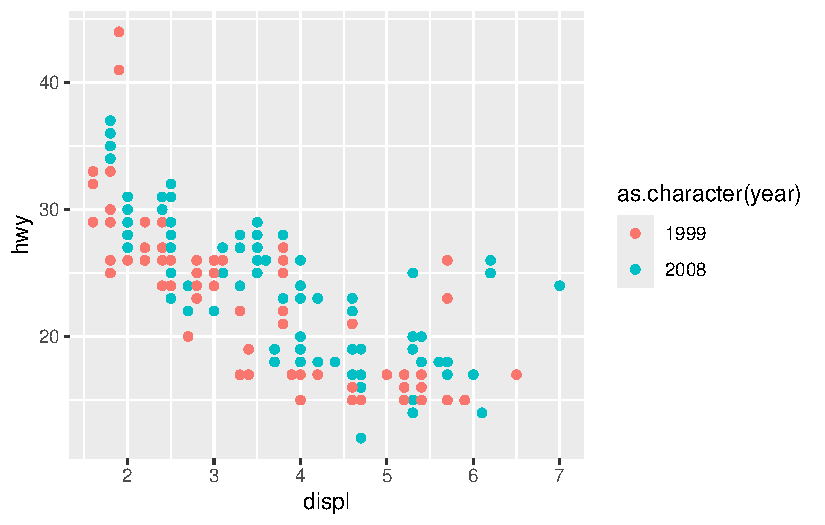
\includegraphics{Part1_Lecture1_Ex_files/figure-pdf/unnamed-chunk-30-1.pdf}

}

\end{figure}

\begin{Shaded}
\begin{Highlighting}[]
\CommentTok{\# or}

\NormalTok{my\_mpg }\OtherTok{\textless{}{-}}\NormalTok{ mpg}
\NormalTok{my\_mpg}\SpecialCharTok{$}\NormalTok{year }\OtherTok{\textless{}{-}} \FunctionTok{as.character}\NormalTok{(my\_mpg}\SpecialCharTok{$}\NormalTok{year)}

\FunctionTok{ggplot}\NormalTok{(}\AttributeTok{data =}\NormalTok{ my\_mpg, }
       \AttributeTok{mapping =} \FunctionTok{aes}\NormalTok{(}\AttributeTok{x =}\NormalTok{ displ, }
                     \AttributeTok{y =}\NormalTok{ hwy,}
                     \AttributeTok{color =}\NormalTok{ year)) }\SpecialCharTok{+}
  \FunctionTok{geom\_point}\NormalTok{() }
\end{Highlighting}
\end{Shaded}

\begin{figure}[H]

{\centering 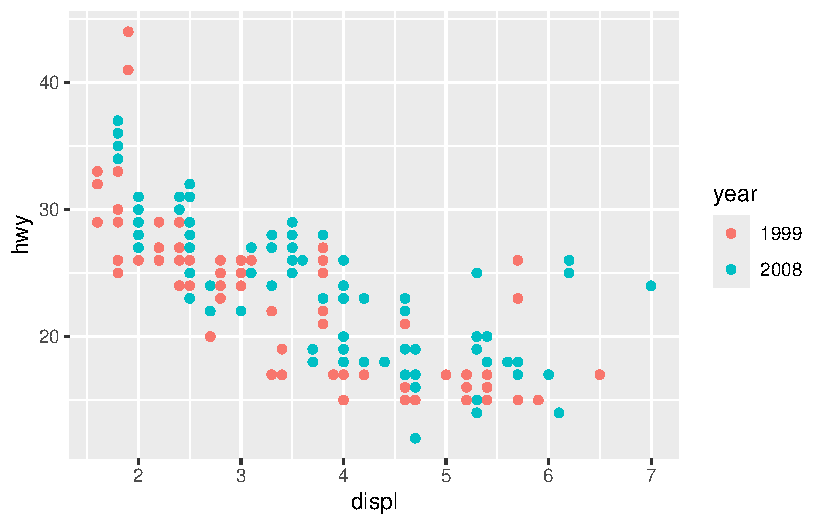
\includegraphics{Part1_Lecture1_Ex_files/figure-pdf/unnamed-chunk-30-2.pdf}

}

\end{figure}

Overlay the scatterplot of my\_mpg with a smoothed trendline using
geom\_smooth. Make sure that only *one* trendline is diplayed.

Make your plot interactive using ggplotly().

\begin{Shaded}
\begin{Highlighting}[]
\NormalTok{my\_mpg }\OtherTok{\textless{}{-}}\NormalTok{ mpg}
\NormalTok{my\_mpg}\SpecialCharTok{$}\NormalTok{year }\OtherTok{\textless{}{-}} \FunctionTok{as.character}\NormalTok{(my\_mpg}\SpecialCharTok{$}\NormalTok{year)}

\FunctionTok{ggplot}\NormalTok{(}\AttributeTok{data =}\NormalTok{ my\_mpg, }
       \AttributeTok{mapping =} \FunctionTok{aes}\NormalTok{(}\AttributeTok{x =}\NormalTok{ displ, }
                     \AttributeTok{y =}\NormalTok{ hwy)) }\SpecialCharTok{+}
  \FunctionTok{geom\_point}\NormalTok{(}\AttributeTok{mapping =} \FunctionTok{aes}\NormalTok{(}\AttributeTok{color =}\NormalTok{ year)) }\SpecialCharTok{+} 
  \FunctionTok{geom\_smooth}\NormalTok{()}
\end{Highlighting}
\end{Shaded}

\begin{verbatim}
`geom_smooth()` using method = 'loess' and formula = 'y ~ x'
\end{verbatim}

\begin{figure}[H]

{\centering 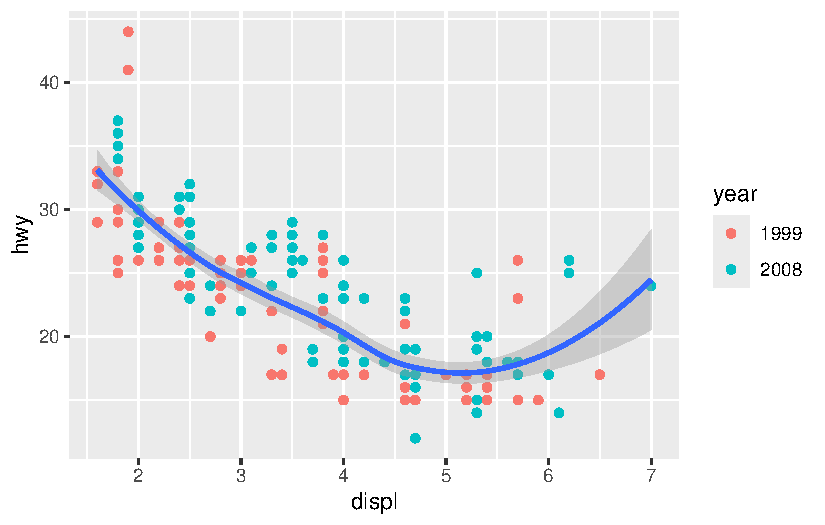
\includegraphics{Part1_Lecture1_Ex_files/figure-pdf/unnamed-chunk-31-1.pdf}

}

\end{figure}

\begin{Shaded}
\begin{Highlighting}[]
\FunctionTok{ggplotly}\NormalTok{(my\_mpg)}
\end{Highlighting}
\end{Shaded}

\begin{verbatim}
Error in UseMethod("ggplotly", p): nicht anwendbare Methode für 'ggplotly' auf Objekt der Klasse "c('tbl_df', 'tbl', 'data.frame')" angewendet
\end{verbatim}

Now create facets of this plot along the discrete variable year, but
don't make it interactive for now.

\begin{itemize}
\item
  Remark: Notice that year is used twice here. Though color-coding year
  is not necessary here, it still helps to stress this variable.

  Now create facets of this plot along the discrete variable drv
  (instead of year).

  Next create facets of this plot along the discrete variable
  manufacturer (instead of drv).

  What can you read out of these facet plots? Do some of them catch your
  eye?
\end{itemize}

\emph{Solution:}

\emph{1) jeep, mercury and nissan look weird: the grey band around the
trendline is very broad. It is the 95\%-confidence interval around the
trendline: a true observation will lie within this band around the
trendline prediction with a probability of 95\%. It thus means that
there is a lot of uncertainty involved in producing the trendline. (We
don't know why yet, but we will come back to that later.)}

\emph{2) lincols, pontiac and subaru look weird as well: its not clear
why no trendline is shown at all. (We will come back to this as well!)}

\emph{3) volkswagen is also bit weird. It makes an unmotivated dip at
approximately x=2 that does not seem to correspond to any of the data
points shown. (We will see the reason later.)}

\begin{Shaded}
\begin{Highlighting}[]
\NormalTok{my\_mpg }\OtherTok{\textless{}{-}}\NormalTok{ mpg}
\NormalTok{my\_mpg}\SpecialCharTok{$}\NormalTok{year }\OtherTok{\textless{}{-}} \FunctionTok{as.character}\NormalTok{(my\_mpg}\SpecialCharTok{$}\NormalTok{year)}

\NormalTok{my\_plot }\OtherTok{\textless{}{-}} \FunctionTok{ggplot}\NormalTok{(}\AttributeTok{data =}\NormalTok{ my\_mpg, }
       \AttributeTok{mapping =} \FunctionTok{aes}\NormalTok{(}\AttributeTok{x =}\NormalTok{ displ, }
                     \AttributeTok{y =}\NormalTok{ hwy)) }\SpecialCharTok{+}
  \FunctionTok{geom\_point}\NormalTok{(}\AttributeTok{mapping =} \FunctionTok{aes}\NormalTok{(}\AttributeTok{color =}\NormalTok{ year)) }\SpecialCharTok{+} 
  \FunctionTok{geom\_smooth}\NormalTok{()}

\NormalTok{my\_plot }\SpecialCharTok{+} \FunctionTok{facet\_wrap}\NormalTok{(}\SpecialCharTok{\textasciitilde{}}\NormalTok{ year)}
\end{Highlighting}
\end{Shaded}

\begin{figure}[H]

{\centering 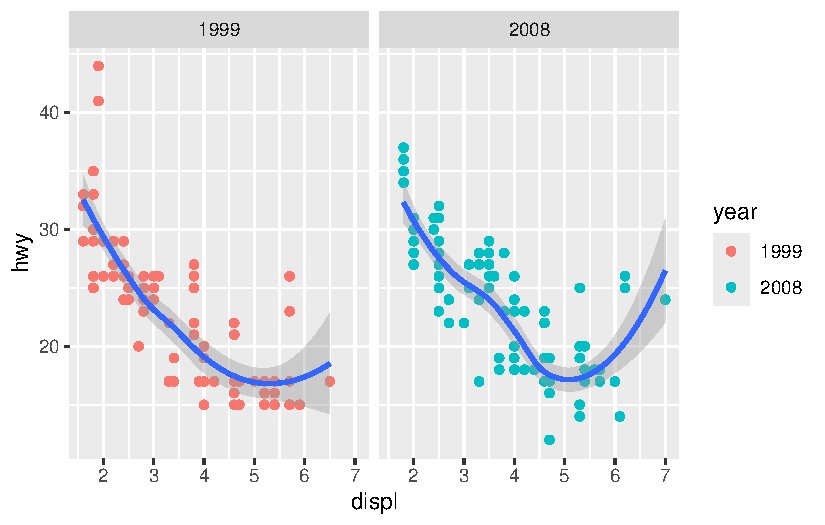
\includegraphics{Part1_Lecture1_Ex_files/figure-pdf/unnamed-chunk-32-1.pdf}

}

\end{figure}

\begin{Shaded}
\begin{Highlighting}[]
\NormalTok{my\_plot }\SpecialCharTok{+} \FunctionTok{facet\_wrap}\NormalTok{(}\SpecialCharTok{\textasciitilde{}}\NormalTok{ drv)}
\end{Highlighting}
\end{Shaded}

\begin{figure}[H]

{\centering 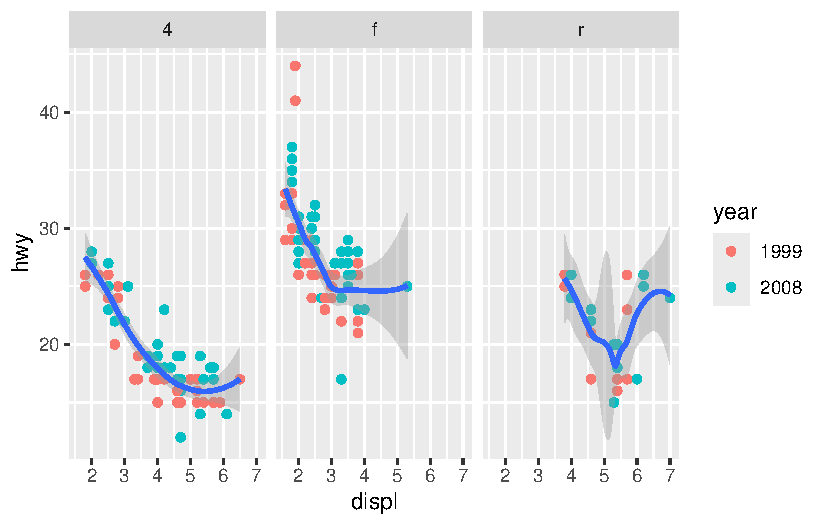
\includegraphics{Part1_Lecture1_Ex_files/figure-pdf/unnamed-chunk-32-2.pdf}

}

\end{figure}

\begin{Shaded}
\begin{Highlighting}[]
\NormalTok{my\_plot }\SpecialCharTok{+} \FunctionTok{facet\_wrap}\NormalTok{(}\SpecialCharTok{\textasciitilde{}}\NormalTok{ manufacturer)}
\end{Highlighting}
\end{Shaded}

\begin{figure}[H]

{\centering 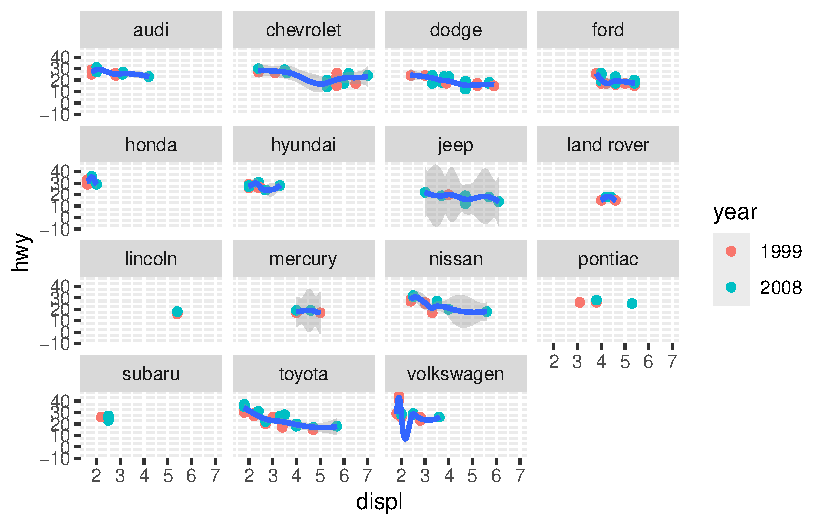
\includegraphics{Part1_Lecture1_Ex_files/figure-pdf/unnamed-chunk-32-3.pdf}

}

\end{figure}

Drop the manufacturer facets again. Instead create a grid of facets
along the discrete variables drv and class.

\begin{Shaded}
\begin{Highlighting}[]
\NormalTok{my\_mpg }\OtherTok{\textless{}{-}}\NormalTok{ mpg}
\NormalTok{my\_mpg}\SpecialCharTok{$}\NormalTok{year }\OtherTok{\textless{}{-}} \FunctionTok{as.character}\NormalTok{(my\_mpg}\SpecialCharTok{$}\NormalTok{year)}

\NormalTok{my\_plot }\OtherTok{\textless{}{-}} \FunctionTok{ggplot}\NormalTok{(}\AttributeTok{data =}\NormalTok{ my\_mpg, }
       \AttributeTok{mapping =} \FunctionTok{aes}\NormalTok{(}\AttributeTok{x =}\NormalTok{ displ, }
                     \AttributeTok{y =}\NormalTok{ hwy)) }\SpecialCharTok{+}
  \FunctionTok{geom\_point}\NormalTok{(}\AttributeTok{mapping =} \FunctionTok{aes}\NormalTok{(}\AttributeTok{color =}\NormalTok{ year)) }\SpecialCharTok{+} 
  \FunctionTok{geom\_smooth}\NormalTok{()}

\NormalTok{my\_plot }\SpecialCharTok{+} \FunctionTok{facet\_grid}\NormalTok{(drv }\SpecialCharTok{\textasciitilde{}}\NormalTok{ class)}
\end{Highlighting}
\end{Shaded}

\begin{figure}[H]

{\centering 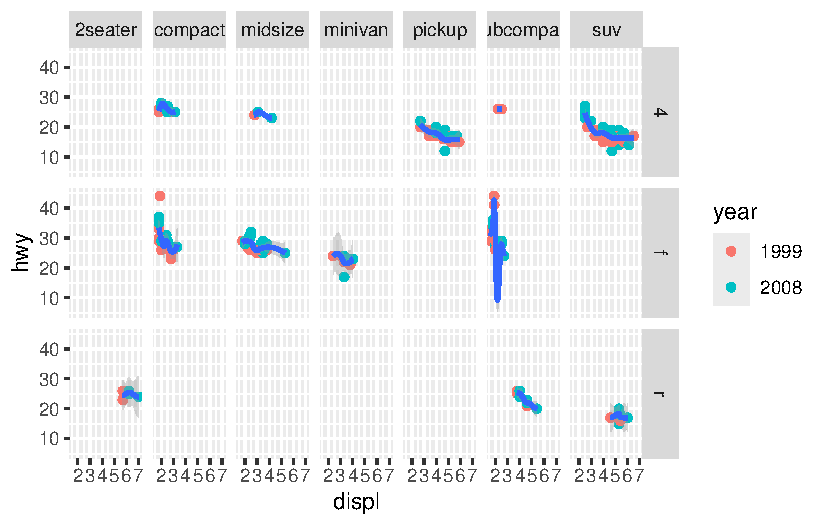
\includegraphics{Part1_Lecture1_Ex_files/figure-pdf/unnamed-chunk-33-1.pdf}

}

\end{figure}

Create a boxplot now that visualizes statistics about the the highway
miles per gallon of the cars in my\_mpg.

\begin{Shaded}
\begin{Highlighting}[]
\NormalTok{my\_mpg }\OtherTok{\textless{}{-}}\NormalTok{ mpg}

\FunctionTok{ggplot}\NormalTok{(}\AttributeTok{data =}\NormalTok{ my\_mpg, }
       \AttributeTok{mapping =} \FunctionTok{aes}\NormalTok{(}\AttributeTok{y =}\NormalTok{ hwy)) }\SpecialCharTok{+}
  \FunctionTok{geom\_boxplot}\NormalTok{() }
\end{Highlighting}
\end{Shaded}

\begin{figure}[H]

{\centering 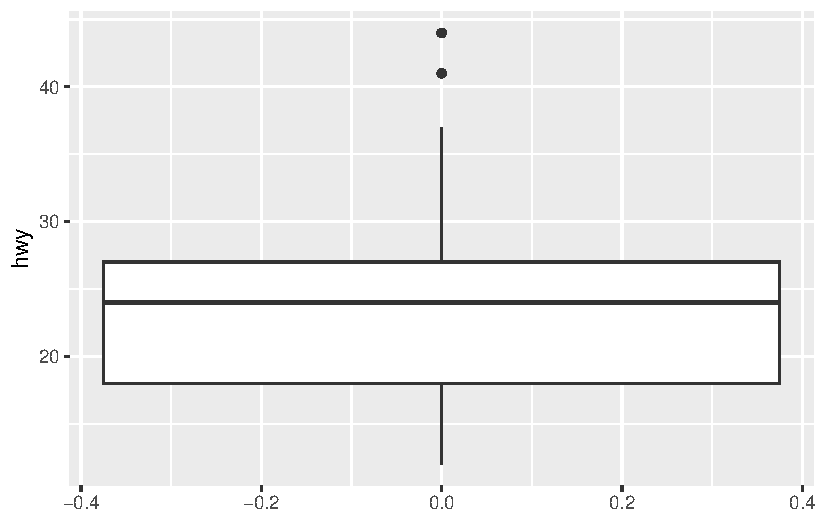
\includegraphics{Part1_Lecture1_Ex_files/figure-pdf/unnamed-chunk-34-1.pdf}

}

\end{figure}

Now make one such boxplot per year (1999 and 2008). Make it interactive.
What can you read out of it?

\emph{Solution: While the median didnt change much, the cars in 2008
show more variability in terms of highway miles per gallon.}

\begin{Shaded}
\begin{Highlighting}[]
\NormalTok{my\_mpg }\OtherTok{\textless{}{-}}\NormalTok{ mpg}

\NormalTok{my\_plot }\OtherTok{\textless{}{-}} \FunctionTok{ggplot}\NormalTok{(}\AttributeTok{data =}\NormalTok{ my\_mpg, }
       \AttributeTok{mapping =} \FunctionTok{aes}\NormalTok{(}\AttributeTok{x =}\NormalTok{ year, }
                     \AttributeTok{y =}\NormalTok{ hwy)) }\SpecialCharTok{+}
  \FunctionTok{geom\_boxplot}\NormalTok{(}\AttributeTok{mapping =} \FunctionTok{aes}\NormalTok{(}\AttributeTok{color =}\NormalTok{ year)) }

\FunctionTok{ggplotly}\NormalTok{(my\_plot)}
\end{Highlighting}
\end{Shaded}

Now create facets of this plot along the variable drv. What new
insight(s) does it give you?

Solution: Most cars with a front-wheel drive are more efficient than
4wds and rwds: they go farther per gallon of gas - independently of the
year of manufacture. Not surprisingly, most 4-wheel drive cars are more
expensive in terms of gas needed per mile than front- or rear wheel
drive cars. Additionally, they show the biggest change from 1999 to 2008
in terms of variability (inter-quartiule range and whiskers).

\begin{Shaded}
\begin{Highlighting}[]
\NormalTok{my\_plot\_fac }\OtherTok{\textless{}{-}}\NormalTok{ my\_plot }\SpecialCharTok{+} \FunctionTok{facet\_wrap}\NormalTok{(}\SpecialCharTok{\textasciitilde{}}\NormalTok{ drv)}

\FunctionTok{ggplotly}\NormalTok{(my\_plot\_fac)}
\end{Highlighting}
\end{Shaded}

Finally let's take a look at ggpairs: Try to create a pairwise variable
plot of mpg using ggpairs().

\begin{Shaded}
\begin{Highlighting}[]
\FunctionTok{ggpairs}\NormalTok{(mpg)}
\end{Highlighting}
\end{Shaded}

\begin{verbatim}
Error in stop_if_high_cardinality(data, columns, cardinality_threshold): Column 'model' has more levels (38) than the threshold (15) allowed.
Please remove the column or increase the 'cardinality_threshold' parameter. Increasing the cardinality_threshold may produce long processing times
\end{verbatim}

We get an error message here! It says that the categorical variable
model has more than 15 levels (i.e.~more than 15 different values),
ggpairs() cannot display more. Check if this is true by typing
length(unique(mpg\$model)).

\begin{itemize}
\item
  Remark: This is what happens here:

  \begin{itemize}
  \item
    mpg\$model addresses only the variable column of the data frame.
  \item
    Remember that every column of a data frame is a vector. We can apply
    the function unique() to see its unique values.
  \item
    The output is again a vector, namely the vector of unique values.
    (You can check with is.vector().)
  \item
    Since unique(mpg\$model) is again a vector, we can apply the
    function length() to count the number of entries.
  \end{itemize}
\end{itemize}

\begin{Shaded}
\begin{Highlighting}[]
\FunctionTok{length}\NormalTok{(}\FunctionTok{unique}\NormalTok{(mpg}\SpecialCharTok{$}\NormalTok{model))}
\end{Highlighting}
\end{Shaded}

\begin{verbatim}
[1] 38
\end{verbatim}

\begin{Shaded}
\begin{Highlighting}[]
\FunctionTok{is.vector}\NormalTok{(}\FunctionTok{unique}\NormalTok{(mpg}\SpecialCharTok{$}\NormalTok{model))}
\end{Highlighting}
\end{Shaded}

\begin{verbatim}
[1] TRUE
\end{verbatim}

The advice in the error message is to exclude the variable model. So
let's do that. You can do that by typing ggpairs(mpg{[},-c(2){]}).
Remark: Don't worry, we will learn how this works a bit later in the
lecture about data frames.

\begin{Shaded}
\begin{Highlighting}[]
\FunctionTok{ggpairs}\NormalTok{(mpg[,}\SpecialCharTok{{-}}\FunctionTok{c}\NormalTok{(}\DecValTok{2}\NormalTok{)]) }
\end{Highlighting}
\end{Shaded}

\begin{figure}[H]

{\centering 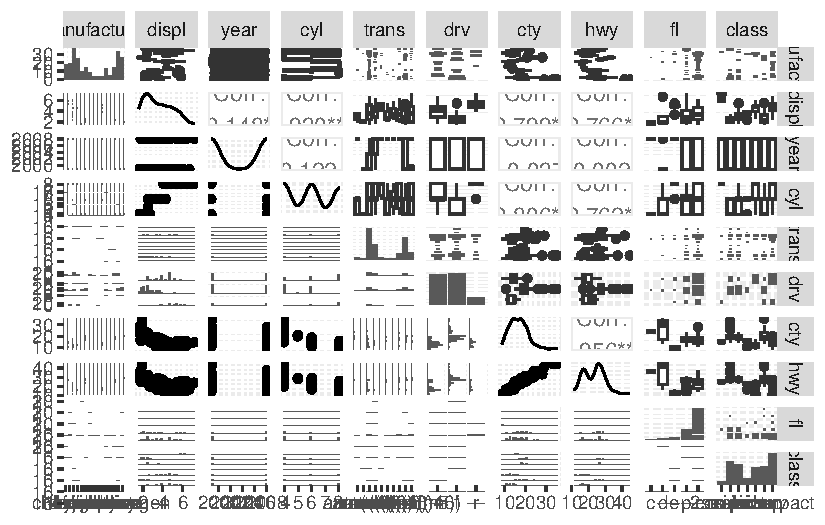
\includegraphics{Part1_Lecture1_Ex_files/figure-pdf/unnamed-chunk-39-1.pdf}

}

\end{figure}

You can now sit down, get a tea and take some time to contemplate this
plot for a bit. Trying to make sense of the different subplots, if you
can. Don't get frustrated if you cannot figure everything out: there is
a lot of information in this plot!

\begin{itemize}
\item
  Remark: The logic is the following:

  \begin{itemize}
  \item
    In the diagonal, there is only one variable to display
    (e.g.~manufacturer). Since it does not make sense to plot
    manufacturer vs manufacturer, a plot type is chosen that is suitable
    for displaying only one variable. If the variable is categorical
    (like manufacturer ), this is a frequency diagram (bar plot). If the
    variable is numerical (like hwy), it is a density plot.
  \item
    In the rest right of the matrix, plot types are chosen that are
    suitable to visualize categorial vs categorical, numerical vs
    numerical or categorical vs numerical variables. Since the upper
    right triangle and the lower left triangle are redundant, different
    plot types are chosen to capture as much info as possible.
  \item
    If you are interested, you can get more info about ggpairs, e.g.,
    here: https://r-charts.com/correlation/ggpairs/ and
    https://www.rdocumentation.org/packages/GGally/versions/2.2.1
  \end{itemize}
\end{itemize}



\end{document}
